%versao de 24-MAR-2019

\chapter{Quantificação nominal}

Neste capítulo, trataremos do valor semântico de expressões como
\textit{alguém}, \textit{ninguém}, \textit{todo mundo}, \textit{algum cachorro}, \textit{um livro},
\textit{nenhuma criança} e \textit{todo professor}. Essas expressões são
chamadas de \textsc{expressões quantificadoras} ou
\textsc{quantificacionais}. Como se pode ver pelas sentenças
abaixo, a exemplo das expressões referenciais que já estudamos nos
capítulos anteriores, as expressões quantificadoras também ocupam,
pelo menos superficialmente, posições argumentais de predicados
verbais e não verbais:


\begin{exe}
    \ex\label{conw}
    \begin{xlist}
        \ex  Alguém dormiu.\label{conwa}
        \ex  Ninguém está em casa.\label{conwz}
        \ex  Todo Mundo ama alguém.\label{conwc}
        \ex  Algum cachorro latiu.\label{conwd}
        \ex  Nenhuma criança gosta do João.\label{conwe}
        \ex  O João entregou um livro pra todo professor.\label{conwf}
    \end{xlist}
\end{exe}

\n  Entretanto, apesar dessa semelhança sintática, expressões
referenciais e expressões quantificadoras devem receber
tratamentos semânticos distintos, conforme veremos já na próxima
seção. No curso da análise que faremos, colocaremos em uso uma
série de recursos já utilizados nos capítulos anteriores, como
atribuições, índices, movimento sintático e regras de mudança
de tipos.

\section{Expressões quantificadoras e indivíduos}

Do ponto de vista sintático, trataremos as expressões
quantificadoras como DPs. Para aquelas sintaticamente complexas,
como \textit{alguma}/\textit{nenhuma}/\textit{toda criança}, assumiremos que os NPs são
complementos dos determinantes (Ds) \textit{alguma}, \textit{nenhuma} e \textit{toda},
respectivamente. Já as expressões \textit{todo mundo}, \textit{alguém} e
\textit{ninguém} serão tratadas como itens lexicais simples, todas elas
pertencentes à categoria D.

\begin{figure}[H]
	\centerline{ \Tree [ [ [ $\left\{\overset{\textstyle \text{Alguma}}{\underset{\textstyle \text{Toda}}{\textstyle \text{Nenhuma}}}\right\}$ ].D [ [ criança ].N ].NP ].DP [ [ dormiu ].V ].VP ].S \hspace{0.5in} \Tree [ [ [ $\left\{\overset{\textstyle \text{Alguém}}{\underset{\textstyle \text{Todo mundo}}{\textstyle \text{Ninguém}}}\right\}$ ].D ].DP [ [ dormiu ].V ].VP ].S } \caption{Sentenças com DPs quantificadores }
\end{figure}


Até o início deste capítulo, já havíamos analisado três tipos de
DPs: descrições definidas, como \textit{o prefeito de Campinas}, nomes
próprios, como \textit{João}, e pronomes, como \textit{ele} ou
\textit{ela}. Para todos eles, atribuímos o tipo semântico $e$ a suas extensões, ou
seja, assumimos que eram indivíduos, membros de D$_{e}$.

A semelhança sintática entre esses DPs e os DPs quantificadores
ilustrados acima pode nos trazer a tentação de analisá-los
semanticamente da mesma forma, ou seja, como expressões
referenciais. Nossa tarefa, nesse caso, seria descobrir a que
indivíduos correspondem as extensões dos DPs quantificadores.

Para o caso de \textit{alguém} ou \textit{algum menino}, a resposta pode parecer
clara: assim como a extensão de \textit{João} é o indivíduo João, a
extensão de \textit{alguém} é também um indivíduo, só que neste caso não
sabemos, ou não revelamos, qual. Podemos chamá-lo simplesmente de
\textit{i}. O mesmo vale para \textit{algum menino}, cuja extensão neste
caso seria um menino \textit{m} qualquer. Conforme mostrado
abaixo, as condições de verdade das sentenças abaixo seriam todas
representadas da mesma forma, variando apenas o indivíduo
atribuído à extensão dos sujeitos:

%xl
\begin{exe}
\ex\label{eee}
\begin{xlist}
	\ex \den{João dormiu} = \den{dormiu}(\den{João}) = 1 \textit{sse} João dormiu.\label{eea}
	\ex \den{Alguém dormiu} = \den{dormiu}(\den{alguém}) = 1 \textit{sse} i dormiu.\label{eeb}
	\ex \den{Algum menino dormiu} = \den{dormiu}(\den{algum menino}) = 1 \textit{sse} m dormiu.\label{eec}
\end{xlist}
\end{exe}

\n Essa semelhança nos leva, entretanto, a certas previsões que não
são confirmadas na prática. Considere, por exemplo, a sentença
(\ref{proj}) abaixo:

\begin{exe}
\ex Não é verdade que Maria esteja namorando João, mas ela está
namorando Pedro.\label{proj}
\end{exe}

\n (\ref{proj}) não é uma contradição, já que o fato de Maria não
estar namorando João é plenamente compatível com o fato de ela
estar namorando Pedro. Considere agora (\ref{proa}):

\begin{exe}
\ex Não é verdade que Maria esteja namorando alguém, mas ela está
namorando Pedro.\label{proa}
\end{exe}

\n (\ref{proa}) soa contraditória, e isso seria esperado se a
primeira parte da sentença fosse interpretada como afirmando que
não existe nenhum indivíduo \textit{x}, tal que Maria esteja
namorando \textit{x}. Isto implica que ela não está namorando o
Pedro, o que contradiz diretamente a segunda parte de
(\ref{proa}). Entretanto, se o que a primeira parte de
(\ref{proa}) afirma é que Maria não está namorando um certo
indivíduo i, cuja identidade não é revelada, ficamos sem uma
explicação de porque (\ref{proa}) soa contraditória, já que ela
não estar namorando um certo indivíduo é plenamente compatível com
ela estar namorando o Pedro, bastando que esse indivíduo não seja
o próprio Pedro.

Considere, agora, as duas inferências abaixo:

\begin{exe}
    \ex João cantou e João dançou. Logo, João cantou e dançou.\label{cd}
    \ex \# Alguém cantou e alguém dançou. Logo, alguém cantou e dançou.
    \label{ce}
\end{exe}

\n Enquanto a inferência em (\ref{cd}) é claramente válida, a
inferência em (\ref{ce}) é claramente inválida, o que indicamos por \# acima. Por exemplo, se
Maria foi a única pessoa que cantou, e Joana a única que dançou,
então estaríamos dizendo a verdade ao dizer que alguém cantou e
alguém dançou, mas estaríamos mentindo se disséssemos que alguém
cantou e dançou. Mas se \textit{alguém} denota um indivíduo, (\ref{ce}),
assim como (\ref{cd}), deveria ser uma inferência válida. Por quê?
Se nos lembrarmos do que vimos sobre coordenação no capítulo 3,
veremos que nosso sistema atribui tanto à premissa quanto à
conclusão em (\ref{cd}) as mesmas condições de verdade, o que é
desejável, já que essas sentenças são, de fato, equivalentes. Mas, se assumirmos que a extensão de \textit{alguém} é também um indivíduo,
seja ele qual for, então estaremos comprometidos com a
equivalência da premissa e da conclusão em (\ref{ce}), o que não é
desejável, já que, como acabamos de ver, essas sentenças não têm as
mesmas condições de verdade.

Vejamos, agora, o caso de \textit{ninguém}. Aqui, já não é nada óbvio que
indivíduo poderia ser a extensão desse item. Mas ainda assim,
assumamos que exista um tipo especial de indivíduo (indivíduo
nulo?) que corresponda à extensão de \textit{ninguém}. Com isso em mente,
considere as inferências abaixo:

%xl
\begin{exe}
\ex\label{pron}
\begin{xlist}
\ex João cantou e dançou. Logo, João cantou e João dançou.\label{prona}
\ex \# Ninguém cantou e dançou. Logo, ninguém cantou e ninguém dançou.\label{pronb}
\end{xlist}
\end{exe}

\n Novamente, não temos um paralelo entre nomes próprios e
sintagmas quantificadores: (\ref{prona}) é válida, mas
(\ref{pronb}) não o é. Para verificar, basta voltar ao nosso
cenário anterior. Nele não havia ninguém que cantou e dançou, mas
havia alguém que cantou e também alguém que dançou. Logo, naquele
cenário, a premissa em (\ref{pronb}) seria verdadeira, mas a
conclusão falsa. Infelizmente, se atribuirmos a \textit{ninguém} um
indivíduo como extensão, nosso sistema atribuirá à premissa e à
conclusão em (\ref{pronb}) as mesmas condições de verdade,
inviabilizando uma explicação para a não validade da
inferência.

Por fim, considerações semelhantes se aplicam à expressão \textit{todo
mundo}, a cuja extensão poderíamos pensar em atribuir um indivíduo
correspondente ao conjunto ou à soma de todos os indivíduos
comuns, como João, Pedro, Maria, etc.

%xl
\begin{exe}
\ex\label{prot}
\begin{xlist}
\ex João comeu peixe ou carne. Logo, João comeu peixe ou João comeu carne.\label{prota}
\ex \# Todo mundo comeu peixe ou carne. Logo, todo mundo comeu peixe ou todo mundo comeu carne.\label{protb}
\end{xlist}
\end{exe}

\n Em um cenário em que metade as pessoas só comeu peixe e a outra metade só comeu carne, a premissa em (\ref{protb}) seria verdadeira, ao passo que a conclusão não, uma vez que nem todo mundo comeu peixe e nem todo mundo comeu carne.

Mais uma vez, temos razões para não identificarmos a extensão de
um sintagma quantificador com um indivíduo, seja ele qual for, justamente pelo comportamento semântico díspar entre as expressões.

\section{Quantificadores generalizados}

Abandonemos então a ideia de tratar as extensões dos sintagmas
quantificadores como indivíduos e busquemos uma alternativa.

Comecemos com a sentença abaixo:

\begin{exe}
    \ex Alguém dormiu. \label{all}
\end{exe}

Intuitivamente, essa sentença é verdadeira se existir um
indivíduo, seja ele quem for, que tenha dormido, e falsa se não
houver nenhum indivíduo que tenha dormido. Nós já sabemos que a extensão do VP
\textit{dormiu} é uma função (tipo $\langle e,t\rangle$) que leva um
indivíduo \textit{x} no valor de verdade 1, se \textit{x} dormiu, e
no valor de verdade 0, se \textit{x} não dormiu. Podemos imaginar
a contribuição de \textit{alguém} para o significado da sentença como um
dispositivo que faz uma busca na extensão de VP e verifica se há
algum indivíduo que é levado ao valor de verdade 1. Se houver, a
sentença será verdadeira. Caso contrário, ela será falsa. Vamos
formalizar essa ideia, atribuindo à extensão de \textit{alguém} o tipo
$\langle\langle e,t\rangle,t\rangle$. A extensão de VP servirá
como argumento para esta função, que retornará o valor de verdade
1, se, e somente se, algum indivíduo no domínio da extensão de VP
for levado ao valor 1.

\begin{exe}
	\ex \den{alguém} = $\lambda F_{\langle e,t\rangle}.\ \exists \textit{x} \in D_{e}\ [F'(x)]$
\end{exe}

\n Uma expressão da forma \underline{$\exists \textit{x} \in\ D_{e}\ [\phi]$} deve ser lida como ``existe um \textit{x} pertencente a $D_{e}$, tal que $\phi$''. O símbolo $\exists$ é tomado emprestado da lógica de predicados e chamado de \textsc{quantificador existencial}. Frequentemente, vamos omitir a informação sobre o domínio, já implícita no uso de variáveis como $x$, $y$ e $z$, na metalinguagem, para membros de $D_{e}$, além de $F$, $G$ e $H$ para funções de tipo $\langle e,t\rangle$. Para obter as condições de verdade de nossa sentença, basta
então que utilizemos aplicação funcional:

\begin{exe}
	\ex \den{Alguém dormiu} = \den{alguém}(\den{dormiu})\\
	= $(\lambda F.\ \exists x[F'(x)])(\lambda x.\ \predica{dormiu}{x})$\\
	= 1 \textit{sse} $\exists x[\predica{dormiu}{x}]$
\end{exe}

Note que semanticamente foi o VP que serviu de argumento ao DP sujeito. Podemos estender o tratamento que acabamos de dar para \textit{alguém} a
\textit{ninguém}. Considere a sentença abaixo:

\begin{exe}
    \ex Ninguém dormiu \label{ni}
\end{exe}

A contribuição de \textit{ninguém} pode ser vista como um dispositivo que
faz uma busca na extensão de VP e verifica se há algum indivíduo
que é levado ao valor de verdade 1. Se não houver, a sentença será
verdadeira. Caso contrário, ela será falsa:\\

\begin{exe}
	\ex \den{ninguém} = $\lambda F.\ \neg\exists x [ F'(x)]$
\end{exe}

\n A expressão \underline{$\neg\exists \textit{x}$} deve ser lida como ``é falso que exista um \textit{x}''. A derivação das condições de verdade de (\ref{ni}) procede da
seguinte forma:

\begin{exe}
	\ex \den{Ninguém dormiu} = \den{ninguém}(\den{dormiu}) \\
	= $(\lambda F.\ \neg\exists x[F'(x)])(\lambda x.\ \predica{dormiu}{x})$\\
	= 1 \textit{sse} $\neg\exists \textit{x}[\predica{dormiu}{x}]$
\end{exe}

\n Note as condições de verdade opostas de \textit{Ninguém dormiu} e
\textit{Alguém dormiu}. Isso reflete a nossa intuição de que se uma
dessas sentenças for verdadeira, a outra será falsa e vice-versa.

O quantificador \textit{todo mundo} pode ser tratado nessa mesma linha.
Para que a sentença \textit{Todo mundo dormiu} seja verdadeira, é preciso
que todos os membros de $D_{e}$ sejam levados ao valor de verdade 1
pela extensão do VP \textit{dormiu}, ou seja, para todo indivíduo
\textit{x}, é preciso que \textit{x} tenha dormido. A entrada
lexical abaixo capta esta intuição:

\begin{exe}
	\ex \den{todo mundo} = $\lambda F.\ \forall x [F'(x)]$
\end{exe}

A expressão \underline{$\forall x$}, também oriunda da lógica de predicados, deve ser lida como ``para todo \textit{x}'', sendo $\forall$ conhecido como \textsc{quantificador universal}. A derivação a seguir mostra como as condições de verdade de
\textit{Todo mundo dormiu} são obtidas através de aplicação
funcional:

\begin{exe}
	\ex \den{Todo mundo dormiu} = \den{todo mundo]}(\den{dormiu})\\
	= $(\lambda F.\ \forall x [F'(x)])(\lambda x.\ \predica{dormiu}{x})$\\
	= 1 \textit{sse} $\forall x [ \predica{dormiu}{x}]$
\end{exe}

Oferecemos, assim, um tratamento uniforme aos itens \textit{ninguém},
\textit{alguém} e \textit{todo mundo}. Todos foram tratados como funções do tipo
$\langle\langle e,t\rangle,t\rangle$. Funções deste tipo são
conhecidas na literatura como \textsc{quantificadores
generalizados}.

\section{Determinantes quantificadores}

Comparemos o significado dos pares de sentenças abaixo:

%xl
\begin{exe}
\ex\label{nin}
\begin{xlist}
\ex Ninguém dormiu.\label{nina}
\ex Nenhum menino dormiu.\label{ninb}
\end{xlist}
\end{exe}

%xl
\begin{exe}
\ex\label{alg}
\begin{xlist}
\ex Alguém dormiu.\label{alga}
\ex Algum menino dormiu.\label{algb}
\end{xlist}
\end{exe}

%xl
\begin{exe}
\ex\label{tod}
\begin{xlist}
\ex Todo mundo dormiu.\label{toda}
\ex Todo menino dormiu.\label{todb}
\end{xlist}
\end{exe}

Vamos começar com as sentenças em (\ref{nin}). Para que
(\ref{nina}) seja verdadeira, é necessário que não haja nenhum
indivíduo que tenha dormido, caso contrário a sentença será falsa. Já
(\ref{ninb}) é menos exigente. Para que ela seja verdadeira, basta
que nenhum menino tenha dormido, ou seja, não deve haver nenhum
indivíduo que seja ao mesmo tempo um menino e que tenha dormido. O
fato de haver ou não meninas ou adultos que tenham dormido é
irrelevante neste caso. As condições de verdade de (\ref{ninb})
podem ser representadas da seguinte forma:

\begin{exe}
	\ex \den{(\ref{ninb})} = 1 \textit{sse} $\neg\exists x [\predica{menino}{x}\ \&\ \predica{dormiu}{x}]$
\end{exe}

\n Para que obtenhamos esse resultado composicionalmente a partir
das extensões do DP \textit{nenhum menino} e do VP \textit{dormiu}, basta que
modifiquemos minimamente a extensão proposta mais acima para
\textit{ninguém}:

\begin{exe}
	\ex \den{nenhum menino} = $\lambda F.\ \neg\exists x [\predica{menino}{x}\ \& \ F'(x)]$
\end{exe}

Assim como no caso de \textit{ninguém}, a extensão de \textit{nenhum menino} é
também um quantificador generalizado, ou seja, uma função de tipo
$\langle\langle e,t\rangle,t\rangle$. Para VP, não há nada de novo
a ser dito. Sua extensão é de tipo $\langle e,t\rangle$:

\begin{exe}
	\ex \den{dormiu} = $\lambda x.\ \predica{dormiu}{x}$
\end{exe}

\n Utilizando aplicação funcional, chegamos ao resultado
desejado:

\begin{exe}
	\ex \den{Nenhum menino dormiu} = \den{nenhum menino}(\den{dormiu})\\
	= $(\lambda F.\ \neg\exists x [ x\ \predica{menino}{x}\ \& \ F'(x)])(\lambda x.\ \predica{dormiu}{x})$\\
	= 1 \textit{sse} $\neg\exists x [ \predica{menino}{x}\ \& \ \predica{dormiu}{x}]$
\end{exe}

Vejamos agora como obter a extensão de \textit{nenhum menino} a partir de
seus constituintes imediatos: o NP \textit{menino} e o determinante
\textit{nenhum}. Já sabemos que a extensão do NP é de tipo $\langle
e,t\rangle$. Acabamos de propor que a extensão do DP é de tipo
$\langle\langle e,t\rangle,t\rangle$. Se quisermos utilizar
aplicação funcional para obter a extensão de DP, só nos resta uma
alternativa para o tipo semântico de D: $\langle\langle
e,t\rangle,\langle\langle e,t\rangle,t\rangle\rangle$, ou, de
maneira simplificada, $\langle et,\langle
et,t\rangle\rangle$:

\begin{figure}[H]
	\centerline{ \Tree [ [ [ nenhum ].\ \ \ \ \ \ \ \ \ \ \ \ \ \textbf{D$_{\langle et,\langle et,t\rangle\rangle}$} [ menino ].\ \ \ \ \ NP$_{\langle et\rangle}$ ].\ \ \ \ \ \ \ DP$_{\langle et,t\rangle}$ \qroof{dormiu}.\ \ \ \ \ VP$_{\langle et\rangle}$ ].\ S$_{\text{t}}$ } \caption{Tipos semânticos em uma sentença com determinante quantificador }
\end{figure}


\n Em termos informais, o que a extensão de \textit{nenhum}\ faz é o
seguinte: ela olha para a extensão de NP e, em seguida, para a extensão de VP, verificando se existe algum indivíduo que é levado ao valor de
verdade 1 tanto pela extensão de NP quanto pela extensão de VP. Se
não houver, a sentença será verdadeira. Se houver, ela será falsa.
Em termos formais, temos o seguinte:

\begin{exe}
	\ex \den{nenhum} = $\lambda F.\ \lambda G.\ \neg\exists x [F'(x)\ \& \ G'(x)]$
\end{exe}

\n Observando o tipo semântico dessa extensão do determinante ($\langle et,\langle et,t\rangle\rangle$), nota-se uma semelhança com o tipo das extensões dos verbos transitivos, como \textit{amar} ($\langle e,\langle e,t\rangle\rangle$). Enquanto a extensão de um verbo transitivo mapeia dois indivíduos (tipo $e$) em um valor de verdade, a de um determinante mapeia duas funções (tipo $\langle e,t\rangle$) em um valor de verdade. Assim como as extensões dos verbos transitivos podem ser vistas como relações entre indivíduos, as dos determinantes podem ser vistas como relações entre funções. Essas relações costumam ser chamadas de \textsc{relações de segunda ordem}, distinguindo-se das \textsc{relações de primeira ordem} associadas aos verbos transitivos.

Prosseguindo na interpretação composicional dos DPs, podemos utilizar aplicação funcional:

\begin{exe}
	\ex \den{nenhum menino} = \den{nenhum}(\den{menino})\\
	= $(\lambda F.\ \lambda G.\ \neg\exists x [F'(x)\ \& \ G'(x)])(\llbracket \text{NP} \rrbracket)$\\
	= $\lambda G.\ \neg \exists x [ \predica{menino}{x}\ \& \ G'(x)]$
\end{exe}

Para postularmos extensões para os determinantes \textit{algum} e \textit{todo},
procedemos de maneira análoga à que acabamos de ver para o caso de
\textit{ninguém}. Comparando o significado de (\ref{alga}) com o de
(\ref{algb}), podemos observar que, enquanto a primeira é
verdadeira sempre que houver algum indivíduo que esteja acordado,
a segunda é mais exigente, precisando haver algum menino acordado.
Intuitivamente, o que a extensão de \textit{algum} parece fazer é olhar
para as extensões de NP e de VP e verificar se existe um indivíduo
que é levado ao valor de verdade 1 tanto pela extensão de NP
quanto pela extensão de VP. Se houver, a sentença será verdadeira,
caso contrário será falsa.

\begin{exe}
	\ex \den{algum} = $\lambda F.\ \lambda G.\ \exists x [ F'(x)\ \& \ G'(x)]$
\end{exe}

Para o caso do determinante \textit{todo}, se compararmos o significado de (\ref{toda}) com o de
(\ref{todb}), notaremos que as condições de verdade da segunda são
menos exigentes que as da primeira. Em termos informais, o que a
extensão de \textit{todo} faz é olhar para as extensões de NP e de VP e
verificar se todo indivíduo levado ao valor de verdade 1 pela
extensão de NP é também levado ao valor de verdade 1 pela extensão
de VP. Somente em caso afirmativo a sentença será
verdadeira:

\begin{exe}
	\ex \den{todo} = $\lambda F.\ \lambda G.\ \forall x [F'(x) \rightarrow G'(x)]$
\end{exe}

\n A expressão $\forall x [ F'(x) \rightarrow G'(x)]$ deve ser lida como ``para todo $x$, se $F(x)$ for igual a 1, então $G(x)$ será igual a 1.'' A derivação das condições de verdade de \textit{Todo menino dormiu} está esquematizada abaixo:

\begin{exe}
	\ex \den{todo menino} = \den{todo}(\den{menino})\\
	= $(\lambda F.\ \lambda G.\ \forall x [F'(x) \rightarrow G'(x)])(\llbracket \text{NP} \rrbracket)$\\
	= $\lambda G.\ \forall x [ \predica{menino}{x}\ \rightarrow G'(x)]$
\end{exe}

\begin{exe}
	\ex \den{Todo menino dormiu} = \den{ Todo menino}(\den{dormiu})\\
	= $(\lambda G.\ \forall x [\predica{menino}{x}\ \rightarrow \ G'(x)])(\lambda x.\ \predica{dormiu}{x})$\\
	= 1 \textit{sse} $\forall x [\predica{menino}{x}\ \rightarrow \predica{dormiu}{x}]$
\end{exe}

Antes de finalizar essa seção, um breve interlúdio técnico sobre a notação que empregamos acima na representação da extensão de \textit{todo}. Essa representação fez uso do símbolo $\forall$, o quantificador universal, que já havíamos visto, e do símbolo $\rightarrow$, conhecido na lógica como \textsc{implicação material} ou simplesmente \textsc{implicação}. Esse símbolo conecta duas fórmulas $\phi$ e $\psi$, sendo $\phi \rightarrow \psi$ lida como ``$\phi$ implica $\psi$'', ou ``se $\phi$, então $\psi$''. Assim como o \& que utilizamos para a coordenação aditiva de sentenças, $\rightarrow$ é definido na lógica como um conectivo verifuncional, com o valor de verdade de $\phi \rightarrow \psi$ dependendo apenas dos valores de verdade de $\phi$ e $\psi$. Mais precisamente, sua contribuição costuma ser representada como na tabela \ref{tabelase}:

\begin{table}
	\begin{tabularx}{.4\textwidth}{XXX}
		\lsptoprule
		$\phi$ & $\psi$ & $\phi\ \&\ \psi$ \\
		\midrule 
		1 & 1 & \ \ \ 1 \\  
		1 & 0 & \ \ \ 0 \\ 
		0 & 1 & \ \ \ 1 \\ 
		0 & 0 & \ \ \ 1 \\
		\lspbottomrule
	\end{tabularx}
	\caption{Tabela de verdade de $\rightarrow$}
	\label{tabelase}
\end{table}



\n Pela tabela acima, nota-se que $\phi \rightarrow \psi$ só será falsa no caso de $\phi$ (chamado de \textsc{antecedente}) ser verdadeiro e $\psi$ (chamado de \textsc{consequente}) ser falso. Daí a paráfrase, se $\phi$, então $\psi$. A ideia é que a verdade do antecedente leve à verdade do consequente. O que pode parecer estranho na tabela acima são as duas últimas linhas. Elas nos informam que se o antecedente for falso, a implicação será sempre verdadeira, independentemente da verdade ou falsidade do consequente. Para o nosso propósito, que é a representação da extensão do determinante quantificador \textit{todo} vista mais acima, isso significa que em um cenário em que não houvesse meninos, a sentença \textit{todo menino dormiu} seria verdadeira. De fato, essa não parece uma consequência desejável. Tampouco seria o seu oposto, ou seja, assumir que a implicação seja falsa nesses casos. Talvez caiba aqui uma análise pressuposicional em que sentenças da forma [todo NP VP] só tenham valor de verdade quando a extensão de NP levar ao menos um indivíduo ao valor 1. Ou, talvez, essas sentenças requeiram uma combinação de recursos semânticos e pragmáticos de modo que seu uso apropriado imponha condições sobre a extensão de NP. No restante deste capítulo, manteremos a entrada lexical vista mais acima para \textit{todo}, deixando de lado essas (importantes) complicações (mas ver as sugestões de leitura ao final do capítulo). 

\section{De volta aos nomes próprios e às descrições definidas}

Já vimos mais acima que não parece uma boa ideia tratar as
extensões de DPs quantificadores como indivíduos. Vamos aqui percorrer o caminho oposto e tentar a unificação dos tipos semânticos
dos DPs, assumindo que nomes próprios e descrições definidas, a
exemplo dos DPs quantificadores, são também de tipo
$\langle\langle e,t\rangle,t\rangle$. Em outras palavras, vamos investigar a
possibilidade de tratarmos nomes próprios e descrições definidas
como quantificadores generalizados. Posteriormente, tiraremos vantagem dessa unificação.

Considere os exemplos abaixo:

\begin{exe}
	\ex João dormiu.\label{jj}
	\ex O prefeito de Campinas dormiu.\label{pp}
\end{exe}

\n A ideia é ver a contribuição do nome próprio João para o
significado de (\ref{jj}) como um dispositivo que olha para a
extensão do VP \textit{dormiu} e verifica se o indivíduo João é levado ou
não ao valor de verdade 1. Se for, então a sentença será
verdadeira. Se não for, a sentença será falsa. Formalizaremos esta
ideia, assumindo a seguinte extensão para \textit{João}:

\begin{exe}
	\ex \den{João} = $\lambda F_{\langle e,t\rangle}.\ F'(\textit{joão})$
\end{exe}

\n As condições de verdade de (\ref{jj}) são obtidas através de
aplicação funcional. Neste caso, a extensão de VP é que serve de
argumento para a extensão do nome próprio:

\begin{exe}
	\ex \den{João dormiu} = \den{João}(\den{dormiu}) \\
	= $(\lambda F.\ F'(\textit{joão}))(\lambda x.\ \predica{dormiu}{x})$\\
	= 1 \textit{sse} $\predica{dormiu}{joão}$
\end{exe}

\n Essas são, claro, as mesmas condições que já havíamos obtido
anteriormente, tratando as extensões dos nomes próprios como
indivíduos (tipo \textit{e}).


A sentença (\ref{pp}) pode ser tratada de maneira semelhante. A
extensão de \textit{o prefeito de Campinas} toma a extensão do VP
\textit{dormiu} como argumento e retorna o valor de verdade 1 se, e
somente se, o único indivíduo que é prefeito de Campinas tiver
dormido.

\begin{exe}
	\ex \den{[o prefeito de Campinas]} = $\lambda F.\ F'(\iota x [\predica{prefeito}{x,Campinas}])$
\end{exe}

As condições de verdade de (\ref{pp}) são obtidas de maneira
idêntica à que acabamos de ver para (\ref{jj}). Já a extensão do
artigo definido precisa ser modificada de acordo, uma vez que, agora, esse
será tratado como os determinantes quantificadores \textit{algum},
\textit{nenhum} e \textit{todo}. Seu novo tipo semântico será $\langle et,\langle
et,t\rangle\rangle$:

\begin{exe}
	\ex $\llbracket \text{o} \rrbracket = \lambda F:\exists !x [F'(x)].\ \lambda G.\ G'(\iota y [F'(y)])$
\end{exe}

\n Note que esta entrada lexical preserva a análise
pressuposicional que havíamos adotado anteriormente para o artigo
definido. Para obter as condições de verdade de (\ref{pp}),
utilizamos aplicação funcional duas vezes. Primeiro para obter a
extensão de DP, a partir de D e NP. Depois para obter a extensão
de S, a partir de DP e VP:

\begin{exe}
	\ex \den{o prefeito de Campinas} = \den{o}(\den{prefeito de Campinas})\\
	\den{(\ref{pp})} = \den{o prefeito de Campinas}(\den{dormiu})
\end{exe}

\n Os detalhes da derivação ficam para o leitor como exercício,
que poderá observar a adequação das condições de verdade obtidas.

A conclusão a que chegamos é que é possível tratar uniformemente a
extensão de nomes próprios, descrições definidas e DPs
quantificadores como sendo quantificadores generalizados. Como já anunciamos, veremos mais adiante uma vantagem que essa unificação traz. Antes, porém, vamos aumentar nosso estoque de quantificadores
generalizados.

\section{Outros DPs quantificadores}

Vejamos, agora, outros DPs cujas extensões podem ser analisadas como
quantificadores generalizados, bem como os determinantes que são
seus núcleos. Considere as sentenças abaixo:

\begin{exe}
    \ex Três meninos dormiram. \label{car}
    \ex Mais de três meninos dormiram. \label{cas}
    \ex Menos de três meninos dormiram. \label{cat}
\end{exe}

\n Comecemos por (\ref{car}), para a qual atribuiremos a seguinte estrutura:

\begin{figure}[H]
	\centerline{ \Tree [.S [.DP [.D três ] [.NP [.N meninos ] ] ] [.VP [.V dormiram ] ] ] } \caption{sentença com um determinante numeral }
\end{figure}


\n Vamos assumir que o plural na forma verbal \textit{dormiram}
resulta de uma regra sintática de concordância sujeito-verbo que
não afeta a interpretação do verbo e que, portanto, a extensão de
\textit{dormiram} é a mesma de \textit{dormiu}. Vamos assumir, ainda, que o plural no nome \textit{meninos} também resulta de uma
regra sintática de concordância, desta vez entre um determinante D e
o NP que é seu complemento. Portanto, estamos assumindo que a
extensão de \textit{meninos} é igual à extensão de
\textit{menino}.

Figurativamente, podemos pensar na extensão do DP \textit{três
meninos} como um contador que verifica o número de meninos que são
levados pela extensão de VP ao valor de verdade 1. Se esse número
for três, a sentença será verdadeira. Se o número for diferente de
três, a sentença será falsa. Para formalizar essa ideia, vamos
lançar mão do conceito de cardinalidade da teoria dos conjuntos. Como estaremos lidando apenas com conjuntos finitos, definiremos a cardinalidade de um conjunto como o número de elementos pertencentes ao conjunto. Usaremos a notação $\mid C \mid$ para representar a cardinalidade de um conjunto $C$ qualquer. Com isso em mente, considere a extensão abaixo:

\begin{exe}
	\ex \den{três meninos} = $\lambda F.\ \mid\{x | \predica{menino}{x}\}\cap\{x | F'(x)\}\mid\ =\ 3$
\end{exe}

\n Essa extensão é um quantificador generalizado, tipo $\langle
et,t\rangle$, que, ao tomar uma função \textit{F} como argumento,
retorna o valor de verdade 1 se, e somente se, a intersecção do
conjunto dos meninos com o conjunto dos indivíduos levados por
\textit{F} ao valor 1 tiver três elementos. Lembre-se de que esse último conjunto é o conjunto caracterizado pela função $F$ e que, conforme decidimos no capítulo 2, representamos por $F_{C}$:

\begin{exe}
	\ex \den{três meninos} = $\lambda F.\ \mid\{x | \predica{menino}{x}\}\cap F_{C}\mid\ =\ 3$
\end{exe}


\n Vamos verificar a
adequação dessa extensão calculando as condições de verdade de
(\ref{car}). Como a extensão de VP é de tipo $\langle e,t\rangle$,
podemos nos valer de aplicação funcional:

\begin{exe}
	\ex \den{três meninos dormiram} = \den{DP}(\den{VP}) \\
	= $(\lambda F.\ \mid\{x | \predica{menino}{x}\}\cap F_{C}\mid\ =\ 3)(\lambda x.\ \predica{dormiu}{x})$\\
	= 1 \textit{sse} $\mid \{x | \predica{menino}{x}\}\cap\{x | \predica{dormiu}{x}\}\mid\ =\ 3$
\end{exe}

\n As condições acima nos dizem que (\ref{car}) é verdadeira se, e
somente se, a interseção do conjunto dos meninos com o conjunto
dos indivíduos que dormiram tiver três elementos. Isso é
exatamente o que queríamos.

Para completar nossa análise da interpretação de (\ref{car}),
precisamos definir a extensão do determinante \textit{três}. Dado o que já
vimos nas seções anteriores sobre o tipo semântico de outros
determinantes quantificadores e o que acabamos de ver sobre a
extensão do DP \textit{três meninos}, nossa tarefa se torna
simples:

\begin{exe}
	\ex \den{três} = $\lambda F.\lambda G.\ \mid F_{C}\cap G_{C}\mid\ =\ 3$
\end{exe}

\n Em palavras, o determinante \textit{três}, após tomar duas
funções \textit{F} e \textit{G} como argumentos, retornará o valor
1 se, e somente se, o número de elementos da intersecção do
conjunto caracterizado por \textit{F} com o conjunto caracterizado
por \textit{G} for igual a três. As duas funções em questão são as
extensões do NP que é complemento de D e do VP do qual o DP
resultante é sujeito.

Esse tratamento se estende imediatamente aos exemplos (\ref{cas})
e (\ref{cat}) acima. Do ponto de vista sintático, vamos
simplificar e assumir que as expressões \textit{mais de três} e
\textit{menos de três} correspondem a itens lexicais (obviamente, isso é apenas uma simplificação, mas foge ao escopo deste livro uma análise morfossintática mais refinada dessas expressões):

\begin{figure}[H]
	\centerline{ \Tree [.S [.DP [.D $\left\{\textstyle\text{mais de três}\atop\textstyle\text{menos de três}\right\}$ ] [.NP [.N meninos ] ] ] [.VP [.V dormiram ] ] ] } \caption{sentença com um determinante contendo um numeral modificado }
\end{figure}


\begin{exe}
	\ex \den{mais de três} = $\lambda F.\lambda G.\ \mid F_{C}\cap G_{C}\mid\ >\ 3$
	\ex \den{menos de três} = $\lambda F.\lambda G.\ \mid F_{C}\cap G_{C}\mid\ <\ 3$
\end{exe}

O leitor deve ter em mente que essa nossa breve incursão na semântica dos numerais (modificados ou não) apenas arranha a superfície de um terreno vasto e complexo. Há usos predicativos e argumentais desses numerais que certamente não se encaixam no que acabamos de ver. Sentenças como \textit{Os três meninos chegaram} ou \textit{Três é um número primo} exigem um tratamento diferente. Além disso, mesmo os casos que apresentamos acima têm sido objeto de controvérsias semânticas que não estamos abordando aqui (ver as sugestões de leitura).


A análise dos numerais como determinantes cardinais pode ser extendida para o indefinido
plural \textit{alguns}. Para que uma sentença como (\ref{due})
seja verdadeira, é preciso que mais de um menino tenha dormido, ou
seja, a interseção do conjunto dos meninos com o conjunto dos
indivíduos que dormiram deve ter mais de um elemento.

\begin{exe}
    \ex Alguns meninos dormiram. \label{due}
	\ex \den{alguns meninos} = $\lambda F.\ \mid \{x | \predica{menino}{x}\}\cap F_{C}\mid\ >\ 1$
	\ex \den{alguns} = $\lambda F.\lambda G\ \mid F_{C}\cap G_{C}\mid\ >\ 1$
\end{exe}


\n Outros DPs cujas extensões podem ser tratadas adequadamente como quantificadores generalizados são expressões da forma \textit{a maioria dos NP}, como na sentença abaixo:

\begin{exe}
    \ex A maioria dos meninos dormiu. \label{mai}
\end{exe}

\n Aqui vamos nos esquivar da análise interna destas expressões,
limitando nossa atenção ao DP como um todo. Para que (\ref{mai})
seja verdadeira, é preciso que o número de meninos que dormiram
seja superior ao número de meninos que não dormiram. Desse modo,
garantimos que mais da metade dos meninos dormiu, que é o que
desejamos. Novamente, serviremo-nos do conceito de cardinalidade:

\begin{exe}
	\ex \den{a maioria dos meninos} = \\
	$\lambda F.\ \mid \llbracket \text{meninos} \rrbracket_{C}\cap F_{C}\mid\ >\ \mid \llbracket \text{meninos} \rrbracket_{C}\cap \overline{F_{C}}\mid $
\end{exe}

\n Lembre-se que $\overline{F_{C}}$ é o complemento de $F_{C}$, o conjunto caracterizado por $F$. De maneira mais geral, temos que:

\begin{exe}
	\ex \den{a maioria dos NP} = $\lambda F.\ \mid \llbracket \text{NP} \rrbracket_{C}\cap F_{C}\mid\ >\ \mid \llbracket \text{NP} \rrbracket_{C}\cap \overline{F_{C}}\mid $
\end{exe}

\n E se, simplificadamente, tratarmos \textit{a maioria dos} como um determinante que toma um NP por complemento, teríamos:

\begin{exe}
	\ex \den{a maioria dos} = $\lambda F.\ \lambda G.\ \mid F_{C}\cap G_{C}\mid\ >\ \mid F_{C}\cap \overline{G_{C}}\mid $
\end{exe}

\n Fica a cargo do leitor verificar a adequação desta extensão,
calculando as condições de verdade de (\ref{mai}).


\section{Coordenação de DPs}

Discutimos mais acima como tratar as extensões de nomes próprios e
descrições definidas como quantificadores generalizados. Isto
permitiu uma unificação dos DPs no que diz respeito ao tipo
semântico de suas extensões: todas elas são de tipo $\langle
et,t\rangle$. Uma vantagem dessa unificação é que ela torna
possível uma análise para a coordenação de DPs baseada no que já
estudamos no capítulo sobre coordenação e, sobretudo, na entrada
lexical que propusemos para o conectivo \textit{e}. Para entender
como, considere as seguintes sentenças:

\begin{exe}
    \ex João e Maria tiraram 10 na prova. \label{de}
    \ex Maria e alguns meninos tiraram 10 na prova. \label{df}
    \ex Dois meninos e três meninas tiraram 10 na prova. \label{dg}
    \ex O filho do João e algumas meninas tiraram 10 na prova. \label{dh}
    \ex Maria e o filho do João tiraram 10 na prova. \label{di}
\end{exe}

\n Como mostram os exemplos acima, é possível coordenar dois tipos
quaisquer de DPs, sejam eles nomes próprios, descrições definidas
ou DPs quantificadores como os que vimos nas seções acima. O
resultado é um outro DP, que, nos exemplos acima, funciona como
sujeito do VP \textit{tiraram 10 na prova}. Antes de passarmos à
análise desses DPs, note que todas as sentenças acima podem ser
parafraseadas por sentenças envolvendo coordenação sentencial:

\begin{exe}
    \ex João tirou 10 na prova e Maria tirou 10 na prova. \label{dde}
    \ex Maria tirou 10 na prova e alguns meninos tiraram 10 na prova.\label{ddf}
    \ex Dois meninos tiraram 10 na prova e três meninas tiraram 10 na prova.\label{ddg}
    \ex O filho do João tirou 10 na prova e algumas meninas tiraram 10 na prova.\label{ddh}
    \ex Maria tirou 10 na prova e o filho do João tirou 10 na prova.\label{ddi}
\end{exe}

\n Lembre-se, agora, que, no capítulo sobre coordenação e negação, após
notarmos a flexibilidade do conectivo \textit{e} em coordenar
diversos tipos de constituintes, postulamos a seguinte entrada
lexical:

\begin{exe}
	\ex Versão polimórfica da conjun\-ção \textit{e}: \\
	\hspace*{18pt}\underline{Caso básico}: se $a = t$, \\
	\hspace*{30pt}$\llbracket e_{\langle a ,\langle a,a\rangle\rangle}\rrbracket = \lambda p_{t}.\ \lambda q_{t}.\ p=1\ \&\ q=1$ \\ 
	\hspace*{18pt}\underline{Casos derivados}: se $a = \langle a_{1},\langle a_{2}, ... ,\langle a_{n},t\rangle ... \rangle\rangle\ (n\geq 1)$, \\
	\hspace*{30pt} $\llbracket e_{\langle a ,\langle a,a\rangle\rangle}\rrbracket = \lambda f_{a}.\lambda g_{a}.\lambda \gamma_{a_{1}}^{1}.\lambda \gamma_{a_{2}}^{2}...\lambda \gamma_{a_{n}}^{n}.$\\ \hspace*{\fill} $\llbracket e_{\langle t\langle t,t\rangle\rangle}\rrbracket(f_{a}(\gamma_{a_{1}}^{1})(\gamma_{a_{2}}^{2})...(\gamma_{a_{n}}^{n}))(g_{a}(\gamma_{a_{1}}^{1})(\gamma_{a_{2}}^{2})...(\gamma_{a_{n}}^{n}))$
\end{exe}

\n Lembre-se de que tipos booleanos são tipos semânticos que
terminam em \textit{t}, como, por exemplo, $t$, $\langle
et\rangle$, $\langle e,et\rangle$ e $\langle
et,t\rangle$. Esse último é justamente o tipo dos quantificadores
generalizados. Note, ainda, que a entrada lexical acima requer que o
tipo semântico dos elementos coordenados seja idêntico. Isso
também não é problema para nós, já que estamos justamente
argumentando a favor de uma análise que atribui às extensões de
todos os DPs o mesmo tipo semântico. Vejamos então o que a entrada
lexical de \textit{e} nos fornece para a coordenação envolvendo o
tipo semântico $\langle et,t\rangle$.

Assumindo, no esquema acima, que $a = \langle et,t\rangle$ e
efetuando as devidas substituições, obteremos o seguinte
(volte ao capítulo 3 se estiver em dúvida sobre como proceder):

\begin{exe}
	\ex $\llbracket e_{\langle ett ,\langle ett,ett\rangle\rangle}\rrbracket = \lambda P_{\langle et,t\rangle}.\lambda Q_{\langle et,t\rangle}.\lambda F_{\langle et\rangle}.\ P(F) = 1\ \&\ Q(F) = 1$
\end{exe}

\n Vamos ilustrar o uso dessa extensão calculando as condições de
verdade de (\ref{df}), cujo DP sujeito \textit{Maria e alguns
meninos} tem a estrutura (simplificada) abaixo (para os demais
exemplos, basta proceder de maneira análoga):

\begin{figure}[H]
	\centerline{ \Tree [.DP \qroof{Maria}.DP$_1$ [ e \qroof{alguns meninos}.DP$_2$ ] ] } \caption{Coordenação de DPs }
\end{figure}

\begin{exe}
	\ex \den{[e DP$_{2}$]} = \den{e}(\den{DP$_{2}$})\\
	\den{[e DP$_{2}$]} = ($\lambda P.\lambda Q.\lambda F.\ P(F) = 1\ \&\ Q(F) = 1$)(\den{DP$_{2}$})\\
	\den{[e DP$_{2}$]} = $\lambda Q.\lambda F.\ \llbracket\text{DP$_{2}$}\rrbracket(F) = 1\ \&\ Q(F) = 1$
\end{exe}

\begin{exe}
	\ex \den{DP} = \den{[e DP$_{2}$]}(\den{DP$_{1}$})\\
	\den{DP} = $\lambda F.\ \llbracket\text{DP$_{2}$}\rrbracket(F) = 1\ \&\ \llbracket\text{DP$_{1}$}\rrbracket(F) = 1$
\end{exe}

\n Como sabemos que

\begin{exe}
	\ex \den{DP$_{1}$} = $\lambda F.\ F'(maria)$ \\
	\den{DP$_{2}$} = $\lambda F.\ \mid \{x | \predica{menino}{x}\}\cap F_{C}\mid\ >\ 1$
\end{exe}

\n temos que:

\begin{exe}
	\ex \den{DP} = $\lambda F.\ \mid \{x | \predica{menino}{x}\}\cap F_{C}\mid\ >\ 1\ \&\ F'(maria)$
\end{exe}

\n Para obtermos as condições de verdade de nossa sentença, basta
utilizarmos aplicação funcional:

\begin{exe}
	\ex \den{S} = \den{DP}(\den{VP})\\
	\den{VP} = $\lambda x.\ \predica{tirou\_10\_na\_prova}{x}$\\
	\den{S} = 1 \textit{sse} $\mid \{x | \predica{menino}{x}\}\ \cap\ \{x | \predica{tirou\_10\_na\_prova}{x}\}\mid\ >\ 1\ \& $ \\
	\hspace*{\fill} $\predica{tirou\_10\_na\_prova}{maria}$
\end{exe}

\n Essas condições de verdade exigem que Maria tenha tirado 10 na
prova e que mais de um menino tenha tirado 10 na prova. Isso é
exatamente o que queríamos.

Antes de fecharmos esta seção, note o seguinte: ao tratarmos nomes
próprios e descrições definidas como tendo extensões de tipo
$\langle et,t\rangle$ não precisamos necessariamente abandonar
nossas considerações dos capítulos anteriores em que elas eram de
tipo \textit{e}. Ao contrário, temos razões para manter essas
extensões para que continuemos a dar conta de sentenças como
\textit{João ama Maria}, em que a extensão do verbo transitivo é
de tipo $\langle e,et\rangle$, buscando, portanto, dois argumentos
de tipo \textit{e}. Para manter todos esses resultados, podemos
recorrer a um expediente que já utilizamos anteriormente, a saber,
uma regra de mudança de tipos. Nesse caso, nosso alvo são
expressões referenciais, que queremos analisar como tendo duas
possíveis extensões: uma de tipo \textit{e} e outra de tipo
$\langle et,t\rangle$. Vamos, então, manter as extensões de tipo
\textit{e} como básicas e fornecer uma regra que relacione
sistematicamente essas extensões com as extensões de tipo $\langle et,t\rangle$:

\begin{exe}
	\ex Regra de mudança de tipos para expressões referenciais (tipo \textit{e}) \\
	Seja \textit{X} um DP cuja extensão $\alpha$ é de tipo \textit{e}. Mude a extensão de \textit{X} para $\alpha '$, sendo $\alpha '$ de tipo $\langle et,t\rangle$ e definida da seguinte forma: $\alpha' = \lambda F_{\langle et\rangle}.\ F'(\alpha)$
\end{exe}


\n Para o nome próprio \textit{Maria}, por exemplo, a regra acima nos fornece o seguinte:

\begin{exe}
	\ex \den{Maria$_{\langle et,t\rangle}$} = $\lambda F_{\langle et\rangle}.\ F'(\llbracket\text{Maria}_{e}\rrbracket)$\\
	\den{Maria$_{e}$} = $maria$\\
	\den{Maria$_{\langle et,t\rangle}$} = $\lambda F_{\langle et\rangle}.\ F'(maria)$
\end{exe}

\n Preservamos, assim, todos os resultados que obtivemos até aqui no
que diz respeito a nomes próprios e descrições definidas.

Cumpre, por fim, salientar que nem todos os casos de coordenação de DPs são amenos a um tratamento na linha do que vimos nesta seção. Certos predicados admitem (ou até exigem) interpretações ditas plurais ou coletivas que nosso sistema não é capaz de captar. Por exemplo:

\begin{exe}
	\ex Alguns alunos e algumas alunas formaram uma equipe para a olimpíada de matemática da escola.
	
	\ex O professor e alguns alunos se reuniram no pátio da escola.
\end{exe} 

\n Nesses casos, as coordenações dos DPs parecem se comportar de maneira diferente, não sendo parafraseáveis por coordenações sentenciais:

\begin{exe}
	
	\ex Alguns alunos formaram uma equipe para a Olimpíada de Matemática da escola e algumas alunas formaram uma equipe para a Olimpíada de Matemática da escola.
	
	\ex O professor se reuniu no pátio da escola e alguns alunos se reuniram no pátio da escola.
	
\end{exe} 


\n Para entender o que se passa em casos como esses, precisaríamos adentrar a semântica da pluralidade, algo que não faremos neste livro, limitando-nos a sugerir algumas leituras ao final do capítulo.

\section{Conservatividade: um universal semântico}

Considere as duas sentenças abaixo e reflita sobre suas condições
de verdade:


\begin{exe}
    \ex\label{prop}
    \begin{xlist}
        \ex  Alguns alunos da minha turma são funcionários da universidade.\label{propa}
        \ex  Alguns funcionários da universidade são alunos da minha tur\-ma.\label{propc}
    \end{xlist}
\end{exe}

\n Como podemos notar, essas sentenças têm condições de verdade
idênticas, ou seja, não há como uma delas ser verdadeira e a outra
falsa. Isto continua sendo válido se trocarmos os NPs e VPs acima
por outros, desde que mantenhamos a estrutura do par, ou seja, desde
que o NP da primeira sentença corresponda ao VP da segunda e o NP
da segunda corresponda ao VP da primeira:


\begin{exe}
    \ex\label{ch}
    \begin{xlist}
        \ex  Alguns brasileiros são descendentes de
        russos.\label{cha}
        \ex  Alguns descendentes de russos são brasileiros.\label{chc}
    \end{xlist}
\end{exe}

\n Essas equivalências nos dizem algo sobre a extensão do
determinante \textit{alguns}. Imagine duas funções \textit{F} e
\textit{G} quaisquer, e que essas funções sirvam, nessa ordem, de
argumento a \textit{alguns}. As condições de verdade que
obteremos
estão representadas abaixo:

\begin{exe}
	\ex \den{alguns}(\textit{F})(\textit{G}) = 1 \textit{sse} $\mid F_{C} \cap G_{C}\mid\ >\ 1$
\end{exe}

\n Compare agora essas condições de verdade com as condições de
verdade que obteríamos se invertêssemos a ordem dos argumentos do
determinante, ou seja, se a extensão de \textit{alguns} se
aplicasse primeiro a \textit{G} e depois a \textit{F}, sendo
\textit{F} e \textit{G} as mesmas funções imaginadas acima:

\begin{exe}
	\ex \den{alguns}(\textit{G})(\textit{F}) = 1 \textit{sse} $\mid G_{C} \cap F_{C}\mid\ >\ 1$
\end{exe}

\n Não é difícil notar que as duas condições de verdade acima são
idênticas. Isso porque a operação de interseção é comutativa.
Assim, para quaisquer conjuntos \textit{A} e \textit{B}, $ A\cap B
=  B\cap A$. Isso torna a ordem dos argumentos do determinante
\textit{alguns} irrelevante do ponto de vista das condições de verdade. Sempre que isso for verdade para um
determinante \textit{D} qualquer, diremos que \textit{D} é
simétrico. Ou seja, estamos atribuindo uma propriedade formal,
\textsc{simetria}, a um determinante. Essa propriedade pode ser
definida da seguinte forma:

\begin{exe}
	\ex Simetria\\
	Para qualquer determinante \textit{D}, e quaisquer funções \textit{F} e \textit{G} de tipo $\langle e,t\rangle$, \textit{D} é simétrico se, e somente se \den{D}(F)(G) = \den{D}(G)(F)
\end{exe}


\n Outros determinantes simétricos são \textit{nenhum}, todos os
numerais e também os numerais modificados como \textit{mais de
três}, \textit{menos de quatro}, etc. No entanto, nem todos os
determinantes são simétricos. Por exemplo, \textit{todo} não o é,
conforme atesta o par de sentenças a seguir:


\begin{exe}
    \ex\label{tt}
    \begin{xlist}
        \ex  Todo brasileiro é sul-americano.\label{tts}
        \ex  Todo sul-americano é brasileiro.\label{ttt}
    \end{xlist}
\end{exe}

\n Enquanto (\ref{tts}) é verdadeira, (\ref{ttt}) é, obviamente,
falsa.

Desde as primeiras aplicações da teoria dos quantificadores
generalizados voltadas para o estudo das línguas naturais, os
estudiosos da área se perguntam se há propriedades que
caracterizam todos os determinantes de todas as línguas naturais. Nesta seção, vamos olhar para uma das propriedades que se tem
postulado como um universal semântico. Trata-se da propriedade
conhecida como \textsc{conservatividade}.

Para se ter uma ideia mais clara sobre o que é um determinante
\textsc{conservativo}, é conveniente pensar nos argumentos da
extensão de um determinante como sendo conjuntos de indivíduos, em vez de funções que levam indivíduos em valores de verdade. Esta
mudança, claro, é uma mera questão de ponto de vista, já que, como
vimos ao final do capítulo 2, existe uma correspondência biunívoca
entre conjuntos de indivíduos e funções de tipo $\langle
e,t\rangle$. Considere, então, as três sentenças abaixo:

\begin{exe}
    \ex Alguma criança chorou. \label{rec}
    \ex Nenhuma criança chorou. \label{red}
    \ex Toda criança chorou. \label{ree}
\end{exe}

\n Todas essas sentenças são da forma D-NP-VP. Vamos representar
por N o conjunto caracterizado pela extensão dos NPs acima, ou seja, o conjunto das
crianças, e por V o conjunto caracterizado pelas extensões dos VPs, ou seja, o
conjunto dos indivíduos que choraram. Podemos dizer então que
(\ref{rec}) é verdadeira se, e somente se, a interseção de N e V
não for vazia, ou seja, se contiver pelo menos um elemento. Já
(\ref{red}) tem condições de verdade opostas, sendo verdadeira
se, e somente se, a interseção de N e V for o conjunto vazio. Por
fim, (\ref{ree}) é verdadeira se, e somente se, todo elemento de N
também for um elemento de V, ou seja, se N for um subconjunto de
V. Essas considerações podem ser convenientemente representadas em
diagramas como os seguintes, em que o retângulo representa o conjunto
de todos os indivíduos:

\begin{figure}[H]
\centerline{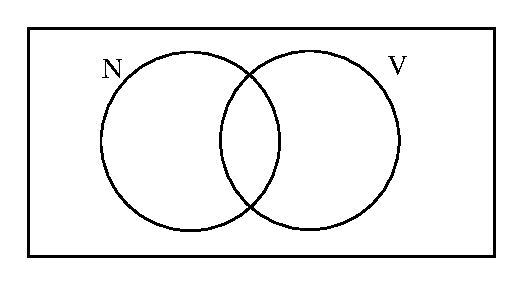
\includegraphics[width=12pc]{figures/algum.eps}}
\caption{Algum: $\text{N}\cap\text{V}\neq\varnothing$}
\end{figure}

\begin{figure}[H]
\centerline{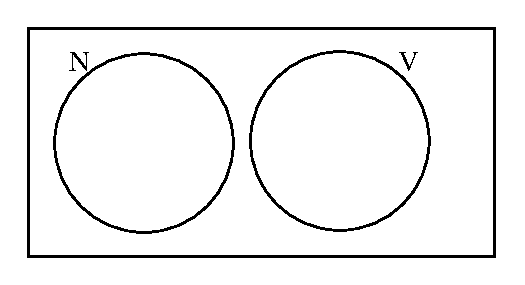
\includegraphics[width=12pc]{figures/nenhum.eps}}
\caption{Nenhum: $\text{N}\cap\text{V}=\varnothing$}
\end{figure}

\begin{figure}[H]
\centerline{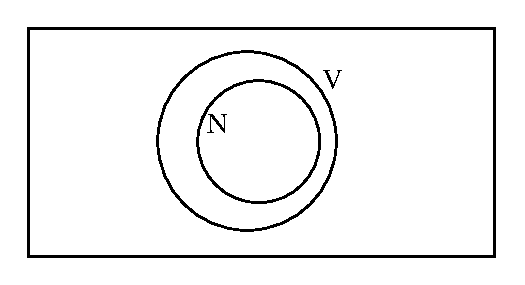
\includegraphics[width=12pc]{figures/todo.eps}} \caption{Todo:
$\text{N}\subseteq\text{V}$}
\end{figure}

\n Note agora uma característica das interpretações das sentenças
(\ref{rec})-(\ref{ree}) relacionada a suas representações acima.
Em todos os casos, para saber se a sentença é verdadeira, basta
perguntar quantos membros do conjunto N são também membros do
conjunto V. As respostas para os exemplos acima, claro, são: pelo
menos um, nenhum e todos, respectivamente. Em nenhum dos casos,
precisamos de informações sobre indivíduos que não pertencem ao
conjunto N. Isto significa que as extensões dos determinantes
acima podem ser caracterizadas levando-se em conta apenas os
conjuntos N e $\text{N}\cap\text{V}$, sem levar em conta os
membros de V que não pertencem a N ou os indivíduos que não
pertencem nem a N nem a V:


\begin{exe}
    \ex\label{lo}
    \begin{xlist}
        \ex  \den{algum}(N)(V) = 1 \textit{sse}
            $\text{N}\cap\text{V}\neq\varnothing$\label{loa}
        \ex  \den{nenhum}(N)(V) = 1 \textit{sse}
            $\text{N}\cap\text{V}=\varnothing$\label{loz}
        \ex  \den{todo}(N)(V) = 1 \textit{sse}
            $\text{N}=\text{N}\cap\text{V}$\label{loc}
    \end{xlist}
\end{exe}

\n Mas se os elementos de V que não estão na interseção com N são mesmo irrelevantes, poderíamos trocar V em (\ref{lo}a-c) por $N \cap V$ sem perda semântica. Considere, então, o que acontece se substituirmos o conjunto V
pelo conjunto $\text{N}\cap\text{V}$ nas condições acima:


\begin{exe}
    \ex\label{clu}
    \begin{xlist}
        \ex  \den{algum}(N)($\text{N}\cap\text{V}$) = 1 \textit{sse}
            $\text{N}\cap (\text{N}\cap\text{V})\neq\varnothing$\label{clua}
        \ex  \den{nenhum}(N)($\text{N}\cap\text{V}$) = 1 \textit{sse}
            $\text{N}\cap (\text{N}\cap\text{V})=\varnothing $\label{cluz}
        \ex  \den{todo}(N)($\text{N}\cap\text{V}$) = 1 \textit{sse}
            $\text{N}=\text{N}\cap (\text{N}\cap\text{V})$\label{cluc}
    \end{xlist}
\end{exe}


\n As condições de verdade acima parecem distintas das anteriores.
Entretanto, pelas definições da teoria dos conjuntos, sabemos que, para quaisquer conjuntos A e B, vale a seguinte equivalência:

\begin{exe}
	\ex $\text{A}\cap (\text{A}\cap\text{B})\ =\ \text{A}\cap\text{B}$
\end{exe}

\n Isso nos permite simplificar as condições de verdade acima, reduzindo-as ao seguinte:


\begin{exe}
    \ex\label{sel}
    \begin{xlist}
        \ex  \den{algum}(N)($\text{N}\cap\text{V}$) = 1 \textit{sse}
            $\text{N}\cap\text{V}\neq\varnothing$\label{sela}
        \ex  \den{nenhum}(N)($\text{N}\cap\text{V}$) = 1 \textit{sse}
            $\text{N}\cap \text{V}=\varnothing$\label{selz}
        \ex  \den{todo}(N)($\text{N}\cap\text{V}$) = 1 \textit{sse}
            $\text{N}=\text{N}\cap\text{V}$\label{selc}
    \end{xlist}
\end{exe}

\n Mas o que aparece à direita do conectivo \textit{sse} nas
condições em (\ref{sel}) é exatamente o que aparecia à direita desse
conectivo nas condições em (\ref{lo}). Isto quer dizer que:


\begin{exe}
    \ex\label{ul}
    \begin{xlist}
        \ex  \den{algum}(N)(V) = \den{algum}(N)($\text{N}\cap\text{V}$)\label{ula}
        \ex  \den{nenhum}(N)(V) = \den{nenhum}(N)($\text{N}\cap\text{V}$)\label{ulz}
        \ex  \den{todo}(N)(V) = \den{nenhum}(N)($\text{N}\cap\text{V}$)\label{ulc}
    \end{xlist}
\end{exe}

\n Equivalências como essas parecem valer
para todos os determinantes das línguas naturais. Elas podem ser expressas em português por esquemas como os mostrados abaixo, em que o símbolo $\equiv$ indica que duas sentenças são semanticamente equivalentes:

\begin{exe}
	\ex D NP VP $\equiv$ D NP é um NP que VP
\end{exe}

\n Concretamente:

\begin{exe}
	\ex Alguma criança chorou $\equiv$ Alguma criança é uma criança que chorou\\
	Nenhuma criança chorou $\equiv$ Nenhuma criança é uma criança que chorou\\
	Toda criança chorou $\equiv$ Toda criança é uma criança que chorou
\end{exe}

\n E são essas equivalências que estão no cerne da propriedade de
conservatividade, que definimos a seguir:

\begin{exe}
	\ex Conservatividade\\
	Para qualquer determinante \textit{D} e quaisquer conjuntos \textit{A} e \textit{B}, \textit{D} é conservativo se, e somente se, $\llbracket D \rrbracket(A)(B)= \llbracket D \rrbracket(A)(A\cap B)$
\end{exe}


\n Podemos, então, formular a seguinte hipótese para as línguas naturais:

\begin{exe}
	\ex Universal da Conservatividade\\
	Todo determinante é conservativo.
\end{exe}


\n A validade desse universal é algo sujeito a confirmação
empírica. Como possível contraexemplo, considere o item
\textit{só} do português, que aparece em sentenças como (\ref{so})
abaixo:

\begin{exe}
    \ex Só crianças choram. \label{so}
\end{exe}

\n Note uma certa semelhança sintática dessa sentença com as que
analisamos mais acima. A palavra \textit{só} vem seguida de um NP
e o constituinte resultante é o sujeito do VP que o segue. Parece
que estamos, de fato, diante de um determinante. Pensemos agora
nas condições de verdade de (\ref{so}). Para que essa sentença
seja verdadeira, é preciso que ninguém além das crianças chore, ou seja, que todo indivíduo que chore seja uma
criança. Isto nos leva à seguinte entrada lexical para
\textit{só}:

\begin{exe}
	\ex \den{só} = $\lambda F_{\langle et\rangle}.\lambda G_{\langle et\rangle}.\ \forall x [G'(x)\rightarrow F'(x)]$
\end{exe}

\n Já na versão baseada em conjuntos que exploramos acima, podemos
caracterizar as condições de verdade de (\ref{so}) através do
diagrama a seguir:

\begin{figure}[H]
\centerline{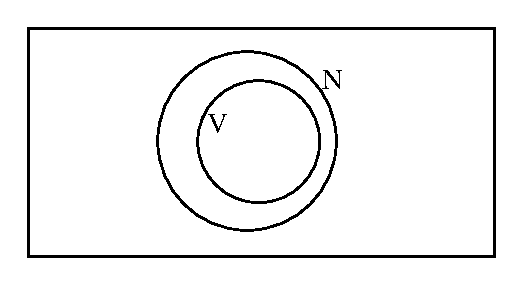
\includegraphics[width=12pc]{figures/so.eps}} \caption{Só:
$\text{V}\subseteq\text{N}$}
\end{figure}

\n Note que, para sabermos se (\ref{so}) é verdadeira, não basta
perguntarmos quantos elementos de N pertencem a V, ou seja, quantas crianças choram. Precisamos
também de informação sobre a existência ou não de elementos que
pertencem a V, mas não pertencem a N. Nesse aspecto, \textit{só}
difere dos determinantes que vimos anteriormente e essa diferença
é fruto do fato de que \textit{só} não é conservativo. 

Para provar a não conservatividade de \textit{só}, basta observar a não equivalência entre \textit{só crianças são crianças que choram} e \textit{só crianças choram}, em oposição à equivalência entre, por exemplo, \textit{toda criança é uma criança que chora} e \textit{toda criança chora}. De um ponto de vista mais formal, basta olharmos para
a caracterização de sua extensão na versão baseada em conjuntos:

\begin{exe}
	\ex \den{só}(N)(V) = 1 \textit{sse} $\text{V}\subseteq\text{N}$
\end{exe}

\n Note que o que aparece do lado direito do conectivo
\textit{sse} é uma contingência, ou seja, algo que pode ser
verdadeiro ou falso dependendo da natureza de \textit{N} e
\textit{V}. Considere agora o que acontece se substituirmos
\textit{V} por
$\text{N}\cap\text{V}$:

\begin{exe}
	\ex \den{só}(N)($\text{N}\cap\text{V}$) = 1 \textit{sse} $(\text{N}\cap\text{V})\subseteq\text{N}$
\end{exe}

\n O que aparece agora após o conectivo \textit{sse} é uma
tautologia, já que, para quaisquer conjuntos \textit{N} e
\textit{V}, a interseção de \textit{N} e \textit{V} é um
subconjunto de N. A conclusão que tiramos disso é que as duas
condições de verdade acima não são equivalentes, e que, portanto,
\textit{só} não é conservativo.

Essa conclusão bastaria para refutarmos o Universal da
Conservatividade, não fosse o fato de que há sólidas evidências de
que \textit{só} não é um determinante. Ao contrário dos
determinantes que discutimos anteriormente, \textit{só} não
precede apenas NPs, mas também DPs, como em \textit{só o menino}
ou \textit{só algumas meninas}, VPs como em \textit{João só
dançou}, APs como em \textit{João está só triste} e PPs, como em
\textit{João viaja só de primeira classe}. Isto leva a crer que \textit{só} é
na verdade um tipo de adjunto que não é seletivo em relação à
categoria do constituinte ao qual se adjunge. Podemos assim manter
viva a hipótese de que determinantes são universalmente
conservativos.

Como já afirmamos acima, universais como esse são hipóteses a serem
confirmadas empiricamente, e uma das linhas de pesquisa abertas
pelo estudo formal das propriedades dos determinantes e dos
quantificadores generalizados que eles originam é justamente a
busca desses universais semânticos.

\section{Quantificação e escopo}

\subsection{DPs quantificadores em posição de objeto}

Todos os exemplos que analisamos até aqui neste capítulo continham
sintagmas quantificadores na posição de sujeito. Tal escolha não
se deu por acaso, e para entender o porquê de termos evitado
outras posições sintáticas, vamos considerar um exemplo com um DP
quantificador na posição de objeto direto de um verbo
transitivo, como em (\ref{tr}):

\begin{exe}
    \ex O João elogia todo professor. \label{tr}
\end{exe}

\n A extensão do verbo \textit{elogia} é de tipo $\langle
e,et\rangle$ e a do DP \textit{todo professor} de tipo $\langle
et,t\rangle$. Não há, portanto, como utilizar aplicação funcional
para obter a extensão do VP \textit{elogia todo professor}.
Outras regras composicionais que introduzimos, como
abstração funcional ou conjunção funcional,
também não nos servem. Essa situação contrasta com casos em que um
DP aparece na posição de sujeito como em (\ref{su}) abaixo, em que
a extensão do VP \textit{elogia o João} é de tipo $\langle e,t\rangle$ e pode servir de argumento para a extensão do DP
sujeito, como já vimos anteriormente:

\begin{exe}
    \ex Todo professor elogia o João. \label{su}
\end{exe}

\n Note que as condições de verdade tanto de (\ref{tr}) quanto de (\ref{su}) são intuitivamente claras e facilmente representáveis na notação que estamos adotando:

\begin{exe}

\ex \den{O João elogia todo professor} = 1 \textit{sse} \\
$\forall x [ \predica{professor}{x}\ \rightarrow\ \predica{elogia}{joão,x}]$ \label{comp1}

\ex \den{Todo professor elogia o João} = 1 \textit{sse} \\
$\forall x [\predica{professor}{x}\ \rightarrow\ \predica{elogia}{x,joão}]$ \label{comp2}

\end{exe}

\n Em ambos os casos, temos o prefixo quantificador $\forall x$ seguido de uma afirmação contendo a variável $x$. Essa afirmação, uma fórmula lógica, é o \textsc{escopo} de $\forall x$. A questão que nos resta é como obter composicionalmente essas condições de verdade no caso de (\ref{comp1}), a começar pelo problema da incompatibilidade de tipos que acabamos de ver.

Logo adiante, veremos como reformular nosso sistema interpretativo e tornar exemplos como (\ref{tr}) interpretáveis, derivando suas condições de verdade sem perder nada do que já obtivemos para casos como (\ref{su}). Antes, porém, vamos discutir dois fenômenos relacionados e que dizem respeito à maneira como DPs quantificadores interagem semanticamente entre si e com a negação.


\subsection{Interação de escopo entre DPs}


Vejamos agora casos em que mais de um DP
quantificador aparece na mesma sentença, como em
(\ref{int}), por exemplo:

\begin{exe}
    \ex Um parecerista anônimo revisará todo artigo que for submetido a esta revista.\label{int}
\end{exe}

\n A primeira coisa a se notar a respeito de
(\ref{int}) é que parecemos estar diante de uma sentença ambígua, que
admite duas interpretações. A primeira interpretação afirma a existência de um certo parecerista que fará a revisão de todos os artigos que forem submetidos ao periódico em questão. De acordo com essa interpretação, para que (\ref{int}) seja verdadeira, é preciso que um único parecerista seja responsável pela revisão de todos os artigos submetidos. Tal interpretação pode ser parafraseada por algo como: existe um parecerista \textit{x}, tal
que \textit{x} revisará todo artigo submetido ao periódico. Ou ainda, e de maneira um pouco mais prolixa: existe um parecerista \textit{x}, tal que, para todo artigo \textit{y} submetido ao periódico, \textit{x} revisará \textit{y}. Usando a notação que empregamos nas seções anteriores, podemos
representar abreviadamente essa interpretação da seguinte maneira:

\begin{exe}
    \ex $\exists x [\predica{parecerista}{x}\ \&\ 
    \forall y [\predica{artigo}{y} \rightarrow \predica{revisará}{x,y}]]$
     \label{qua}
\end{exe}


\n O que está escrito em (\ref{qua}) é que existe um indivíduo
\textit{x} que tem duas propriedades: \textit{x} é parecerista e \textit{x} revisará todo artigo em questão. 

Antes de prosseguir, vamos olhar mais atentamente para a estrutura
interna da representação formal em (\ref{qua}). Olhando de fora
para dentro, notamos que (\ref{qua}) tem a forma $\exists
x [\phi]$, em que $\phi$ é uma fórmula lógica. Essa fórmula é o
escopo do quantificador $\exists x$ introduzido pelo
determinante  \textit{um}. Note agora que no interior de $\phi$
está a contribuição do determinante \textit{todo}, que podemos representar esquematicamente por $\forall y [\psi]$, em que $\psi$ é também uma fórmula lógica. Em casos como esse, dizemos que o quantificador existencial introduzido pelo determinante \textit{um} tem escopo sobre o
quantificador universal introduzido pelo determinante \textit{todo}, ou, vendo de ângulo oposto, que o quantificador universal introduzido pelo determinante \textit{todo} está no escopo do
quantificador existencial introduzido pelo determinante \textit{um}. Pode-se dizer também que o DP sujeito tem escopo sobre o DP objeto.

Passemos agora para a segunda interpretação de (\ref{int}), um
pouco menos saliente que a primeira. De acordo com essa interpretação, todo artigo submetido ao periódico passará pela revisão de um parecerista, não necessariamente o mesmo. Tal interpretação não exige a existência de um certo parecerista que revise todos os artigos em questão. Exige-se apenas que, para todo artigo \textit{y}, exista um parecerista \textit{x}, tal que \textit{x} revise \textit{y}. Formalmente, temos o seguinte:

\begin{exe}
   \ex $\forall y [\predica{artigo}{y} \rightarrow \exists x [\predica{parecerista}{x}\ \&\ 
        \predica{revisará}{x,y}]]$
     \label{xa}
\end{exe}

\n A representação em (\ref{xa}) nos diz que para todo \textit{y}, se \textit{y} é um artigo, então existe um \textit{x}, tal que \textit{x} é um parecerista e \textit{x} revisará \textit{y}. Note
que, aqui, é o quantificador existencial $\exists$ que
aparece no interior da formula introduzida pelo quantificador
universal $\forall$. Dizemos nesse caso que o quantificador universal tem escopo sobre o existencial, ou ainda, que o DP
\textit{todo artigo submetido a este periódico} tem escopo sobre o DP
\textit{um parecerista}.

Analisando as interpretações de (\ref{qua}), deparamo-nos então
com uma \textsc{ambiguidade de escopo} e queremos que nosso sistema interpretativo consiga ajudar a explicá-la.

\subsection{Negação e escopo}

Passemos, agora, a um caso em que um DP quantificador interage com um outro tipo de operador, a negação. Considere a sentença abaixo:

\begin{exe}
    \ex João não elogia todo professor. \label{elo}
\end{exe}

\n Na interpretação mais natural desta sentença, para que ela seja
verdadeira é preciso que haja pelo menos um professor que o João
não elogie. Dito de maneira um pouco mais prolixa, é falso que para todo professor \textit{x}, o João elogia
\textit{x}. Podemos representar essas condições de verdade da
seguinte forma:

\begin{exe}
    \ex $\neg\forall x [\predica{professor}{x}\ \rightarrow\ \predica{elogia}{joão,x}]$ \label{wq}
\end{exe}

\n Para uma fórmula do tipo $\neg\phi$, em que $\phi$ também é uma
fórmula, dizemos que $\phi$ corresponde ao escopo do operador
negativo $\neg$. Para uma fórmula $\forall x [\phi]$, já vimos que $\phi$ é o escopo do quantificador universal $\forall$. Note que, em (\ref{wq}), o quantificador universal aparece no interior do
escopo do operador negativo. Dizemos, então, que a negação tem
escopo sobre o quantificador universal. Costuma-se dizer também que a negação tem escopo sobre o DP quantificador.

Já para uma interpretação de (\ref{elo}) em que o quantificador universal tivesse escopo sobre a negação, teríamos algo parafraseável como ``para todo professor \textit{x}, é falso que o João elogia \textit{x}''. Em termos formais:

\begin{exe}
    \ex $\forall x [\predica{professor}{x} \rightarrow\ \neg\predica{elogia}{joão,x}]$ \label{wqq}
\end{exe}


\n De acordo com (\ref{wqq}), (\ref{elo}) é verdadeira se, e somente se, para qualquer professor \textit{x}, não for verdade que João elogia \textit{x}, ou seja se, e somente se, João não elogiar nenhum professor. Essa parece ser uma interpretação bem menos saliente para (\ref{elo}) e talvez só seja possível quando o DP quantificador estiver bastante enfatizado. De qualquer forma, precisamos ver como nosso sistema interpreta estruturas em que DPs quantificadores e negação estão presentes em uma mesma estrutura.

Nas duas próximas seções, vamos apresentar e discutir, uma de cada vez, duas estratégias para lidar com as questões levantadas nessa seção a respeito da interpretação de DPs quantificadores e seu escopo relativo a outros constituintes sintáticos. A primeira delas é eminentemente sintática, mantendo nosso sistema interpretativo
intacto, mas operando transformações sobre a estrutura sintática das sentenças. Já a segunda, vai na direção oposta,
sendo eminentemente semântica. De acordo com ela, a estrutura
sintática relevante para sua interpretação é a estrutura superficial com DPs quantificadores ocupando as mesmas posições argumentais que DPs referenciais. Porém, os tipos semânticos atribuídos a alguns componentes
da sentença são modificados através de regras de mudanças de tipos. 

\section{Quantificação e movimento}

Voltemos ao caso dos DPs quantificadores em posição de objeto:

\begin{exe}
	\ex O João elogia todo professor. \label{etp}
\end{exe}

\n As condições de verdade dessa sentença exigem que, para todo indivíduo $x$, se $x$ for professor, então $x$ é elogiado pelo João. Na linha do que estamos vendo nesse capítulo, chegaríamos a esse resultado se fornecêssemos à extensão do determinante \textit{todo} funções que caracterizassem o conjunto dos indivíduos que são professores e o conjunto do indivíduos que João elogia. Quanto ao primeiro, não há problema: trata-se da extensão do NP complemento de D. Mas e o segundo? Eis o que queremos:

\begin{exe}
	\ex $\lambda x.\ \predica{elogia}{joão,x}$
\end{exe}
 

A primeira estratégia que veremos consiste em uma operação sintática de movimento. Nela, um DP quantificador se desloca para o topo de uma sentença, deixando para trás um vestígio. Esse DP movido e o seu vestígio recebem índices numéricos idênticos, como representado a seguir (para facilitar a referência a novos nós formados no topo de uma sentença após a operação de movimento, vamos rotulá-los de S$'$, S$''$, etc.):

\begin{figure}[H]
	\centerline{ \begin{forest}
			[S$'$ 
			[DP$_1$[{todo professor},roof,name=subj]]
			[S
			[DP[{o Joao},roof]]
			[VP
			[V[elogia]]
			[t$_1$,name=vest]
			]
			]
			]
			\draw[->] (vest) to[out=south west,in=south] (subj);	
	\end{forest} } \caption{Alçamento de Quantificador }
\end{figure}




\n Essa operação sintática é conhecida como \textsc{alçamento de
quantificador} (AQ) e tem como peculiaridade o fato de que não
afeta a maneira como pronunciamos a sentença, apenas a maneira
como a interpretamos. Em outras palavras, o resultado desta
operação não é visível para o componente fonológico da gramática, apenas
para o componente semântico.

A exemplo do que vimos quando discutimos a estrutura interna das
orações relativas, vamos assumir, \textit{a la} \cite{heikra98}, um processo de transferência de
índices na interface sintaxe-semântica, em que o índice do
constituinte movido é transferido desse para o constituinte que for seu
irmão.

\begin{figure}[H]
	\centerline{ \Tree [.S\2 \qroof{todo professor}.DP [.S\1 1 [.S \qroof{O
			João}.DP [.VP [.V elogia ] t$_1$ ] ] ] ] } \caption{Alçamento de Quantificador e transferência de índice }
\end{figure}



\n Portanto, para a interpretação de (\ref{etp}), é a estrutura
acima que o componente semântico recebe como \textit{input}.
Vejamos, agora, como nosso sistema interpreta essa estrutura. De
acordo com o que vimos no capítulo anterior, quando introduzimos a
regra de abstração funcional, temos que:

\begin{exe}
	\ex \den{S$'$}$^{g}$ = $\lambda x.\ \llbracket\text{S}\rrbracket^{g[1\rightarrow x]}$
\end{exe}

\n Como sabemos que (consulte o capítulo anterior se você tiver dúvidas):

\begin{exe}
	\ex \den{S}$^{g[1\rightarrow x]}$ = 1 \textit{sse} $\predica{elogia}{joão,x}$
\end{exe}

\n então,

\begin{exe}
	\ex \den{S$'$}$^{g}$ = $\lambda x.\ \predica{elogia}{joão,x}$
\end{exe}

\n Isso é exatamente o que queríamos. Note que essa extensão é uma função de tipo $\langle
e,t\rangle$, que é o que a extensão do DP movido toma como
argumento. Podemos, então, utilizar aplicação funcional para obter a extensão de $S''$:

\begin{exe}
	\ex\den{S$''$}$^{g}$ = \den{DP}$^{g}$(\den{S$'$}$^{g}$) \\
	\den{DP}$^{g}$ = $\lambda F.\ \forall x [\predica{professor}{x} \rightarrow\ F'(x)]$\\
	\den{S$''$}$^{g}$ = 1 \textit{sse} $\forall x [\predica{professor}{x} \rightarrow\ \predica{elogia}{joão,x}]$
\end{exe}

\n Note que, como a extensão acima não depende da atribuição
\textit{g} (essa não aparece à direita de \textit{sse}), podemos,
de acordo com a convenção que adotamos no capítulo anterior,
escrever simplesmente:

\begin{exe}
	\ex \den{S$''$} = 1 \textit{sse} $\forall x [\predica{professor}{x} \rightarrow\ \predica{elogia}{joão,x}]$
\end{exe}


\n Essas eram exatamente as condições de verdade que queríamos derivar. Usando apenas princípios composicionais que já tínhamos à disposição, em particular aplicação e abstração funcional, conseguimos derivar o significado de (\ref{etp}). O custo disso, claro, foi a postulação de uma operação sintática (AQ) sem reflexos fonológicos.


\subsection{Movimento e escopo}

A regra de alçamento de quantificadores move um DP quantificador
para o topo da sentença, deixando em seu lugar de origem um
vestígio. Vamos aplicá-la agora ao exemplo com dois DPs quantificadores que vimos anteriormente e que repetimos em
(\ref{rt}):

\begin{exe}
    \ex Um parecerista (anônimo) revisará todo artigo (que for submetido a esta revista).  \label{rt}
\end{exe}

O alvo de AQ será o DP \textit{todo artigo}, o que resultará
na estrutura abaixo (já assumindo a transferência de índice):

\begin{figure}[H]
	\centerline{ \Tree [.S\2$_{t}$ \qroof{todo artigo}.\ \ \ \ \ \ DP\1$_{\langle et,t \rangle}$ [.\ \ \ S\1$_{\langle e,t \rangle}$ 1 [.S$_{t}$ \qroof{um parecerista}.\ \ \ \ \ \ DP$_{\langle et,t \rangle}$ [.\ \ \ \ \ \ \ VP$_{\langle e,t \rangle}$ [.\ \ \ \ \ \ V$_{\langle e,et \rangle}$ revisará ] \ \ \ $t_{1_{e}}$ ] ] ] ] } \caption{Alçamento de quantificador e interação de escopo }
\end{figure}


\n Nessa estrutura, foram anotados os tipos semânticos de todos os nós, de acordo com o previsto pelas entradas lexicais e as regras de aplicação funcional e abstração funcional. Note que não há incompatibilidades e que o nó raiz (S) é de tipo $t$, como deve ser. Vejamos, então, a interpretação que nosso sistema deriva para essa
estrutura, procedendo de cima para baixo. Omitiremos alguns passos, deixando-os a cargo do leitor.

\begin{exe}
	\ex \den{S$''$}$^{g}$ = \den{DP$'$}$^{g}$(\den{S$'$}$^{g}$) \\
	\den{DP$'$}$^{g}$ = $\lambda F.\ \forall x [\predica{artigo}{x}\ \rightarrow\ F'(x)]$\\
	\den{S$''$}$^{g}$ = 1 \textit{sse}  $\forall x [\predica{artigo}{x} \rightarrow\ \llbracket\text{S}'\rrbracket^{g}(x)=1]$
\end{exe}

\n Para o nó S$'$, usamos abstração funcional:

\begin{exe}
	\ex \den{S$'$}$^{g}$ = $\lambda z.\ \llbracket\text{S}\rrbracket^{g[1\rightarrow z]}$
\end{exe}

\n Para evitar confusões nos processos de conversão-$\lambda$ durante a derivação, usamos aqui a variável $z$, já que $x$ e $y$ aparecerão em outros momentos da derivação. Trata-se, entretanto, da mesmíssima regra com a qual já estamos familiarizados. Para o nó S, voltamos a utilizar aplicação funcional:

\begin{exe}
	\ex \den{S}$^{g[1\rightarrow z]}$ = \den{DP}$^{g[1\rightarrow z]}$(\den{VP}$^{g[1\rightarrow z]}$)

	\ex \den{DP}$^{g[1\rightarrow z]}$ = $\lambda F.\ \exists y [\predica{parecerista}{y}\ \&\ F'(y)]$
\end{exe}

\n Por fim, para o nó VP, teremos, via aplicação funcional:

\begin{exe}
	\ex \den{VP}$^{g[1\rightarrow z]}$ = \den{V}$^{g[1\rightarrow z]}$(\den{t$_{1}$}$^{g[1\rightarrow z]}$)\\
	\den{V}$^{g[1\rightarrow z]}$ = $\lambda v.\lambda w.\ \predica{revisará}{w,v}$\\
	\den{t$_{1}$}$^{g[1\rightarrow z]}$ = $g[1\rightarrow z](1)$ = $z$
\end{exe}

\n Note o uso na representação da extensão de V das variáveis $v$ e $w$, diferentes das já utilizadas mais acima. Aqui também o intuito é manter a clareza na exposição da derivação.

Tendo chegado à parte de baixo da estrutura, basta percorrermos o sentido inverso, efetuando as devidas conversões:

\begin{exe}
	\ex \den{VP}$^{g[1\rightarrow z]}$ = $\lambda w.\ \predica{revisará}{w,z}$\\
	\den{S}$^{g[1\rightarrow z]}$ = 1 \textit{sse} $\exists y [\predica{parecerista}{y}\ \&\ \predica{revisará}{y,z}]$\\
	\den{S$'$}$^{g}$ = $\lambda z.\ \exists y [\predica{parecerista}{y}\ \&\ \predica{revisará}{y,z}]$\\
	\den{S$''$}$^{g}$ = 1 \textit{sse} \\
	$\forall x [\predica{artigo}{x} \rightarrow \exists y [\predica{parecerista}{y}\ \&\ \predica{revisará}{y,x}]]$
\end{exe}

\n O que as condições acima requerem é que todo artigo seja revisado por um parecerista, não necessariamente o mesmo. Isso corresponde exatamente à leitura que discutimos na seção anterior em
que o DP \textit{todo artigo} tem escopo sobre o DP
\textit{um parecerista}. De fato, se compararmos as condições de verdade
acima com a representação que atribuímos a essa leitura anteriormente em
(\ref{xa}), notaremos que elas são idênticas, exceto pelas escolhas das variáveis, o que é irrelevante.

Derivamos, assim, uma das interpretações de (\ref{rt}). Mas, e a
outra, que afirma a existência de um certo parecerista que revisará todos os artigos em questão? Note que, na estrutura que gerou as condições de verdade
que acabamos de derivar, o DP \textit{todo artigo} aparece em
uma posição hierarquicamente superior ao DP \textit{um parecerista},
resultando na leitura em que o primeiro tem escopo
sobre o segundo. Para obtermos a leitura em que
\textit{um parecerista} tem escopo sobre \textit{todo artigo}, vamos
aplicar AQ novamente, desta vez movendo o DP \textit{um parecerista}
por sobre o DP \textit{todo artigo}. Isto resultará na seguinte estrutura:

\begin{figure}[H]
	\centerline{ \Tree [.S$''''$ \qroof{um parecerista}.DP [.S$'''$ 2 [.S$''$ \qroof{todo artigo}.DP$'$ [.S$'$ 1 \qroof{t$_{2}$ revisará t$_{1}$}.S ] ] ] ] } \caption{Estrutura após duas aplicações de AQ}
\end{figure}




\n Vejamos, então, que condições de verdade nosso sistema deriva para essa estrutura. Procure acompanhar atentamente cada passo da derivação:

\begin{exe}
	\ex \den{S$''''$}$^{g}$ = \den{DP}$^{g}$(\den{S$'''$}$^{g}$)\\
	\den{S$'''$}$^{g}$ = $\lambda x.\ \llbracket\text{S}''\rrbracket^{g[2\rightarrow x]}$ \\
	\den{S$''$}$^{g[2\rightarrow x]}$ = \den{DP$'$}$^{g[2\rightarrow x]}$(\den{S$'$}$^{g[2\rightarrow x]}$)\\
	\den{S$'$}$^{g[2\rightarrow x]}$ = $\lambda y.\ \llbracket\text{S}\rrbracket^{g[2\rightarrow x][1\rightarrow y]}$ \\
	\den{S}$^{g[2\rightarrow x][1\rightarrow y]}$ = \den{V}$^{g[2\rightarrow x][1\rightarrow y]}$(\den{t$_{1}$}$^{g[2\rightarrow x][1\rightarrow y]}$)(\den{t$_{2}$}$^{g[2\rightarrow x][1\rightarrow y]}$)  \\
	\den{S}$^{g[2\rightarrow x][1\rightarrow y]}$ = 1 \textit{sse} $\predica{revisará}{x,y}$\\
	\den{S$'$}$^{g[2\rightarrow x]}$ = $\lambda y.\ \predica{revisará}{x,y}$\\
	\den{S$''$}$^{g[2\rightarrow x]}$ = \den{DP$'$}$^{g[2\rightarrow x]}$($\lambda y.\ \predica{revisará}{x,y}$)\\
	\den{DP$'$}$^{g[2\rightarrow x]}$ = $\lambda F.\ \forall y [\predica{artigo}{y} \rightarrow F'(y)]$\\
	\den{S$''$}$^{g[2\rightarrow x]}$ = 1 \textit{sse} $\forall y [\predica{artigo}{y} \rightarrow\ \predica{revisará}{x,y}]$\\
	\den{S$'''$}$^{g}$ = $\lambda x_{e}.\ \forall y [\predica{artigo}{y} \rightarrow\ \predica{revisará}{x,y}]$\\
	\den{S$''''$}$^{g}$ = \den{DP}$^{g}$($\lambda x.\ \forall y [\predica{artigo}{y} \rightarrow\ \predica{revisará}{x,y}]$)\\
	\den{DP}$^{g}$ = $\lambda F.\ \exists x [\predica{parecerista}{x}\ \&\ F'(x)]$\\
	\den{S$''''$}$^{g}$ = 1 \textit{sse} $\exists x [\predica{parecerista}{x}\ \&\ \forall y [\predica{artigo}{y} \rightarrow\ \predica{revisará}{x,y}]]$
\end{exe}

\n Se compararmos essas condições de verdade com a representação
em (\ref{qua}) apresentada originalmente, veremos que elas são idênticas.
Conseguimos, assim, captar a leitura de (\ref{rt}) em que
\textit{um parecerista} tem escopo sobre \textit{todo artigo}.

Podemos concluir que a regra sintática AQ permite gerar duas
estruturas sintáticas para (\ref{rt}) e que a interpretação de
cada uma delas resulta em uma das leituras associadas a essa
sentença. Explicamos, assim, a ambiguidade de (\ref{rt}),
reduzindo-a a um caso de ambiguidade sintática, em que à mesma
sentença (entendida como uma sequência de palavras) atribuímos
duas estruturas distintas. O custo disso, voltamos a repetir, é a postulação de um nível de representação sintática abstrato e que não corresponde à estrutura superficial da sentença no que diz respeito à posição dos DPs quantificadores.

Cumpre notar também que não impusemos nenhuma restrição a AQ relacionada à natureza dos DPs quantificadores alvejados por ela. Dessa forma, prevemos que sempre que houver dois ou mais deles em uma mesma oração, haverá ambiguidade. Essa liberdade acaba sendo problemática na medida em que certas combinações de DPs não admitem múltiplas interpretações. Considere, por exemplo, o caso abaixo:

\begin{exe}

	\ex Todo mundo resolveu menos de três questões. \label{glu}	
	
\end{exe}

\n Intuitivamente, a única leitura admissível para essa sentença é a de que para todo $x$, $x$ resolveu menos de três questões. Em outras palavras, não deve haver ninguém que tenha resolvido três ou mais questões. Essa é a interpretação em que o quantificador universal introduzido por \textit{todo mundo} tem escopo largo, que inclui a contribuição semântica do DP objeto e que pode ser obtida alçando-se esse último para uma posição sintática subordinada à do DP sujeito:

\medskip

\begin{exe}
	\ex $[$ [$_{\text{DP}}$ \tikzmark{Todo mundo}] 1 [ [$_{\text{DP}}$ \tikzmark{menos de 3} questões] 2 [ \tikzmark{t}$_{1}$ resolve\tikzmark{u} t$_{2}$ ]  ] $]$
	\arrowtop{t}{Todo mundo}
	\arrowbottom{menos de 3}{u}
\end{exe}	

\medskip

Considere, agora, a estrutura resultante do movimento do DP objeto para uma posição acima da do DP sujeito:

\begin{exe}
	\ex $[$ [$_{\text{DP}}$ \tikzmark{menos de 3} questões] 2 [ [$_{\text{DP}}$ \tikzmark{todo mundo}] 1 [ \tikzmark{t}$_{1}$ resolve\tikzmark{u} t$_{2}$ ]  ] $]$
	\arrowtop{t}{todo mundo}
	\arrowbottom{menos de 3}{u}
\end{exe}

\medskip

\n Nesse caso, teremos uma inversão de escopo e a interpretação resultante será a de que menos de três questões foram resolvidos por todo mundo. Mas essa não é uma interpretação que (\ref{glu}) tem. Pensemos um pouco mais a respeito. Imagine, por exemplo um cenário com cinco pessoas (p$_{1}$-p$_{5}$), cinco questões (q$_{1}$-q$_{5}$) e os fatos relevantes representados a seguir:

\begin{exe}
	\ex \begin{tabular}[t]{l l}
		%\hline 
		\textit{pessoas} & \textit{questões resolvidas} \\ 
		%\hline 
		p$_{1}$ &  q$_{1}$,q$_{2}$,q$_{3}$,q$_{4}$,q$_{5}$\\ 
		%\hline 
		p$_{2}$ &  q$_{1}$,q$_{2}$\\ 
		%\hline 
		p$_{3}$ &  q$_{1}$,q$_{2}$,q$_{4}$\\ 
		%\hline 
		p$_{4}$ &  q$_{1}$,q$_{2}$,q$_{5}$\\ 
		%\hline 
		p$_{5}$ &  q$_{1}$,q$_{2}$,q$_{3}$,q$_{4}$\\ 
		%\hline 
	\end{tabular}
\end{exe}

\n Nesse cenário, é falso que todo mundo tenha resolvido menos de três questões. p$_{1}$, por exemplo, resolveu todas as cinco. Mas é verdadeiro que menos de três questões tenham sido resolvidas por todo mundo (apenas duas, q$_{1}$ e q$_{2}$, foram). Se a inversão de escopo fosse possível, (\ref{glu}) deveria ser julgada verdadeira nessas circunstâncias. Como esse não é o caso, concluímos que essa inversão não é possível.

Além disso, parece haver diferenças translinguísticas em alguns casos. O português brasileiro, por exemplo, parece bastante rígido em relação à possibilidade de inversão de escopo. Mesmo em sentenças como as que vimos anteriormente, envolvendo quantificadores universal e existencial, tal inversão parece bem pouco saliente. Deixaremos essas observações como um alerta para o leitor. De alguma forma, AQ (ou qualquer operação que seja responsável pelo movimento dos DPs quantificadores) precisa ter seu papel regulado, com o movimento sintático em questão afetando de maneira distinta,  diferentes tipos de DPs quantificadores. Remetemos o leitor a algumas das sugestões de leitura oferecidas ao final do capítulo. 



\subsection{Negação e alçamento de quantificadores}

Considere novamente a sentença abaixo:

\begin{exe}
    \ex João não elogia todo professor. \label{eloi}
\end{exe}

\n Como já discutimos, a interpretação mais natural dessa sentença exige que seja falso que João elogie todo professor. Vejamos se nosso sistema consegue derivar as condições de
verdade almejadas. Já sabemos que para interpretar um DP
quantificador na posição de objeto direto, precisamos movê-lo para
o topo da sentença. Isso nos fornece a seguinte
estrutura:



\begin{figure}[H]
	\centerline{ \Tree [.S\2 \qroof{todo professor}.DP [.S\1 1 [.S João [.VP$'$ não [.VP elogia t$_1$ ] ] ] ] ] } \caption{AQ e negação}
\end{figure}


\n Calculemos as condições de verdade dessa estrutura:

\begin{exe}
	\ex \den{S$''$}$^{g}$ = \den{DP}$^{g}$(\den{S$'$}$^{g}$)\\
	\den{S$'$}$^{g}$ = $\lambda x_{e}.\ \llbracket\text{S}\rrbracket^{g[1\rightarrow x]}$\\
	\den{S}$^{g[1\rightarrow x]}$ = \den{VP$'$}$^{g[1\rightarrow x]}$(\den{João})$^{g[1\rightarrow x]}$\\
	\den{VP$'$}$^{g[1\rightarrow x]}$ = \den{não}$^{g[1\rightarrow x]}$(\den{VP}$^{g[1\rightarrow x]}$)\\
	\den{VP}$^{g[1\rightarrow x]}$ = \den{elogia}$^{g[1\rightarrow x]}$(\den{t$_{1}$}$^{g[1\rightarrow x]}$)\\
	\den{elogia}$^{g[1\rightarrow x]}$ = $\lambda x.\lambda y.\ \predica{elogia}{y,x}$\\
	\den{t$_{1}$}$^{g[1\rightarrow x]}$ = $x$\\
	\den{VP}$^{g[1\rightarrow x]}$ = $\lambda y.\ \predica{elogia}{y,x}$\\
	\den{não}$^{g[1\rightarrow x]}$ = $\lambda F.\ \lambda z.\ \neg F'(z)$\\
	\den{VP$'$}$^{g[1\rightarrow x]}$ = $\lambda z.\ \neg\predica{elogia}{z,x}$\\
	\den{João}$^{g[1\rightarrow x]}$ = \textit{joão}\\
	\den{S}$^{g[1\rightarrow x]}$ = 1 \textit{sse}  $\neg\predica{elogia}{joão,x}$\\
	\den{S$'$}$^{g}$ = $\lambda x.\ \neg\predica{elogia}{joão,x}$\\
	\den{DP}$^{g}$ = $\lambda F.\ \forall x [\predica{professor}{x} \rightarrow F'(x)]$\\
	\den{S$''$}$^{g}$ = 1 \textit{sse} $\forall x [\predica{professor}{x} \rightarrow \neg\predica{elogia}{joão,x}]$
\end{exe}

\n O que essas condições de verdade requerem é que, para todo
professor \textit{x}, o João não elogie \textit{x}, ou seja, que o
João não elogie nenhum professor. Conforme já salientamos, essa interpretação, se é que
existe, é bem menos saliente que a interpretação de acordo com a qual se nega apenas que o João elogie todo e qualquer professor. O problema com as condições que
acabamos de derivar é que, de acordo com elas, o quantificador
universal tem escopo sobre a negação, enquanto o que queríamos
era que a negação tivesse escopo sobre o quantificador universal.

Mas como obter a interpretação de (\ref{eloi}) que desejamos?
Dado o que já vimos sobre interação de escopo na seção anterior, a
resposta parece simples: basta mover o DP \textit{todo professor}
para uma posição abaixo da negação. Vejamos se isso realmente
funciona. A estrutura que obteríamos seria a seguinte:

\begin{figure}[H]
	\centerline{ \Tree [.S João [. não [.VP\2 \qroof{todo professor}.DP\1 [.VP\1 1 \qroof{elogia t$_{1}$}.VP ] ] ] ] } \caption{AQ sob a negação}
\end{figure}


\n O problema é que essa estrutura não é interpretável. A extensão
de VP é de tipo $\langle e,t\rangle$. Com isso, a extensão de VP$'$
será de tipo $\langle e,et\rangle$, em razão da regra de abstração funcional. Como a extensão de
\textit{todo professor} é de tipo $\langle et,t\rangle$, não há
como derivar a extensão de VP$''$ e, por conseguinte, de nenhum nó
acima dele, incluindo o nó-raiz S. Note que, para tornar VP$''$
interpretável, bastaria que a extensão de VP$'$ fosse de tipo
$\langle e,t\rangle$ e que dessa forma pudesse servir de argumento
para a extensão de \textit{todo professor}. Mas, para isso, a
extensão de VP precisaria ser de tipo \textit{t}, o que
exigiria que o sujeito fosse interpretado no interior de VP,
saturando assim a extensão do verbo \textit{elogiar}.

Para implementar essa possibilidade, vamos nos valer daquilo que,
dentro do quadro teórico conhecido como \textsc{Teoria da regência e
ligação}, é chamado de \textsc{hipótese do sujeito interno a
VP} (ver referências ao final do capítulo). De acordo com essa hipótese, o sujeito de uma sentença é
gerado no interior de VP, movendo-se depois para a posição que
ocupa na estrutura superficial da sentença. Assim como nos outros
casos envolvendo movimento que já estudamos, vamos assumir que, ao se mover, o DP sujeito recebe um índice e deixa em sua posição de
origem um vestígio coindexado. Após o processo da transferência de
índice, obtém-se então a seguinte estrutura:

\begin{figure}[H]
	\centerline{ \begin{forest}
			for tree={s sep=10mm, inner sep=0, l=0}
			[S
			[DP$_{suj}$,name=subj]
			[$\alpha$
			[$i$]
			[\ldots
			[\ldots]
			[VP,circle,draw,fill=lightgray
			[t$_i$,name=vest]
			[V$'$
			[V]
			[DP$_{obj}$]
			]
			]
			]
			]
			]
			\draw[->] (vest) to[out=south west,in=south] (subj);	
	\end{forest} } \caption{Movimento do sujeito interno a VP }
\end{figure}



\n Vamos aplicar essas ideias ao nosso exemplo. Após movermos o sujeito para fora de VP, teremos:

\begin{figure}[H]
	\centerline{ \Tree [.S João [. 1 [. não \qroof{ t$_{1}$ elogia todo professor}.VP ] ] ] } \caption{Negação e sujeito interno a VP }
\end{figure}


Em seguida, movemos o DP objeto para a posição imediatamente abaixo da negação, resultando na seguinte estrutura:

\begin{figure}[H]
	\centerline{ \Tree [.S João [. 1 [. não [. \qroof{todo professor}.DP [. 2 \qroof{ t$_{1}$ elogia t$_{2}$}.VP ] ] ] ] ] } \caption{AQ, negação e sujeito interno a VP }
\end{figure}



\n Eis os principais passos da derivação das condições
de verdade dessa estrutura:

\begin{exe}
	\ex \den{S}$^{g}$ = \den{1 não todo professor 2 VP}$^{g}$(\textit{joão})\\
	\den{1 não todo professor 2 VP}$^{g}$ = $\lambda x.\ \llbracket \text{não todo professor 2 VP}\  \rrbracket^{g[1\rightarrow x]}$\\
	\den{não todo professor 2 VP}$^{g[1\rightarrow x]}$ = \\
	 \hspace*{\fill} \den{não}$^{g[1\rightarrow x]}$(\den{todo professor 2 VP})$^{g[1\rightarrow x]}$\\
	\den{todo professor 2 VP}$^{g[1\rightarrow x]}$ = \den{todo professor}$^{g[1\rightarrow x]}$(2 VP)$^{g[1\rightarrow x]}$\\
	\den{2 VP}$^{g[1\rightarrow x]}$ = $\lambda y.\ \llbracket\text{VP}\rrbracket^{g[1\rightarrow x][2\rightarrow y]}$\\
	\den{VP}$^{g[1\rightarrow x][2\rightarrow y]}$ = 1 \textit{sse} $\predica{elogia}{x,y}$
\end{exe}

\n Note que a extensão de VP é de tipo \textit{t}.
Efetuando-se as devidas substituições e conversões-$\lambda$, obteremos o seguinte:

\begin{exe}
	\ex \den{2 VP}$^{g[1\rightarrow x]}$ = $\lambda y.\ \predica{elogia}{x,y}$ \\
	\den{todo professor 2 VP}$^{g[1\rightarrow x]}$ = 1 \textit{sse} $\forall y [\predica{professor}{y} \rightarrow \predica{elogia}{x,y}]$
\end{exe}

\n Essa última extensão é de tipo $t$. Portanto, para a negação, deve-se usar a versão de tipo $\langle t,t\rangle$, de acordo com a entrada lexical que propusemos no capítulo 3:

\begin{exe}
	\ex \den{não} = $(\lambda p.\ p=0)$
\end{exe}

\n Prosseguindo, teremos:

\begin{exe}
	\ex \den{não todo professor 2 VP}$^{g[1\rightarrow x]}$ \\
	= ($\lambda p.\ p=0$)(\den{todo professor 2 VP})$^{g[1\rightarrow x]}$\\
	 = 1 \textit{sse} \den{todo professor 2 VP}$^{g[1\rightarrow x]}$ = 0 \\
	 = 1 \textit{sse} $\neg\forall y [\predica{professor}{y} \rightarrow \predica{elogia}{x,y}]$\\
	\den{1 não todo professor 2 VP}$^{g}$ = $\lambda x.\ \neg\forall y [\predica{professor}{y} \rightarrow \predica{elogia}{x,y}]$\\
	\den{S} = 1 \textit{sse} $\neg\forall y [\predica{professor}{y} \rightarrow \predica{elogia}{joão,y}]$
\end{exe}

\n Essas são exatamente as condições que queríamos derivar, com a negação tendo escopo sobre o quantificador universal. Novamente, valemo-nos de operações de movimento sintático que preparam, por assim dizer, a estrutura sintática para a interpretação baseada apenas em aplicação e abstração funcional, sem necessidade de rever os tipos semânticos dos constituintes envolvidos.


\section{Quantificação e mudança de tipos}

Vejamos, agora, uma segunda estratégia para a interpretação de
sentenças com DPs quantificadores em diversas posições sintáticas. Como anunciamos mais acima, essa estratégia mantém a
estrutura sintática superficial da sentença inalterada, sem alçamento de DPs quantificadores ou vestígio de sujeito interno a VP. No caso de \textit{O João elogia todo professor}, por exemplo, o que o componente semântico recebe para interpretar é a
estrutura abaixo:

\begin{figure}[H]
	\centerline{ \Tree [.S \qroof{O João}.DP [.VP [.V elogia ] \qroof{todo professor}.DP ] ] } \caption{Estrutura superficial sem movimento nem sujeito interno a VP }
\end{figure}


\n Para evitarmos a incompatibilidade de tipos que já detectamos
entre as extensões de V e do DP objeto, precisamos alterar pelo
menos uma dessas extensões, ou então criarmos um novo princípio
composicional. Vamos aqui implementar a primeira possibilidade, alterando o tipo semântico dos verbos.

Já notamos no início deste capítulo que, do ponto de vista
sintático, existe uma semelhança na distribuição de expressões
referenciais como nomes próprios e a distribuição de DPs
quantificadores, ambos ocupando as mesmas posições junto aos
predicados a eles relacionados. A ideia por trás da implementação
que vamos desenvolver aqui é a de que as extensões dos predicados
estão em sintonia com esses fatos e que regras semânticas podem
alterar o tipo dessas extensões, de modo a
torná-las aptas a tomar não só indivíduos (tipo $e$) mas
também quantificadores generalizados (tipo $\langle et,t\rangle$)
como argumentos. De maneira mais concreta, isso significa que há
regras que relacionam sistematicamente predicados de indivíduos e
predicados de quantificadores generalizados. Vamos aqui tomar os primeiros como básicos e derivar a extensão dos últimos elevando o tipo semântico de seus argumentos de $e$ para $\langle et,t\rangle$ quando necessário. Chamaremos essa regra de \textsc{Elevação de Argumento} (EA).

\begin{exe}
	\ex Elevação de argumento (EA) \\
	Seja \textit{X} um constituinte cuja extensão $\alpha$ é de tipo $\langle a_{1},...\langle a_{k},...\langle a_{n},t\rangle...\rangle\rangle$, com $n \geq 1$ e $a_{k} = e$. Mude a extensão de \textit{X} de $\alpha$ para $\alpha '$, mudando $a_{k}$ de $e$ para $\langle et,t\rangle$ e definindo $\alpha '$ da seguinte forma:\\
	\hspace*{\fill} $\alpha ' = \lambda x_{1}...\lambda Q_{\langle et,t\rangle}...\lambda x_{n}.\ Q(\lambda x_{k}.\ \alpha(x_{1})...(x_{k})...(x_{n}))$
\end{exe}

\n A regra acima aplica-se a funções com \textit{n} argumentos $x_{1},...,x_{k},...,x_{n}$, sendo o k-ésimo desses argumentos ($x_{k}$) de tipo \textit{e}. A regra modifica o tipo desse k-ésimo argumento, passando-o de $e$ para $\langle et,t\rangle$. É esse novo argumento \textit{Q} que será fornecido por um DP quantificador ocupando uma posição argumental. Vejamos um exemplo concreto com o verbo transitivo \textit{elogiar}. A extensão desse verbo é uma função de tipo $\langle e,et\rangle$, que toma dois argumentos de tipo \textit{e}. No esquema acima, portanto, $n=2$ e tanto $a_{1}$ quanto $a_{2}$ são iguais a \textit{e}. Vamos aplicar EA, tomando \textit{k} como sendo igual a $1$, e portanto, $x_{k}$ como sendo o primeiro argumento, que corresponde à posição de objeto direto. Esse argumento terá seu tipo elevado de $e$ para $\langle et,t\rangle$. A nova extensão do verbo será, portanto, de tipo $\langle \langle et,t\rangle,et\rangle$. Lembremos que a extensão original do verbo \textit{elogiar}, de tipo $\langle e,et\rangle$, é:

\begin{exe}
	\ex $\llbracket \text{elogia}_{1} \rrbracket = \lambda x.\lambda y.\ \predica{elogia}{y,x}$
\end{exe}

\n Marcamos o verbo com um subscrito para diferenciar a extensão original da nova extensão que obteremos, aplicando a mudança de tipos especificada acima:

\begin{exe}
	\ex $\llbracket \text{elogia}_{2} \rrbracket = \lambda Q_{\langle et,t\rangle}.\lambda y.\ Q(\lambda x.\ \llbracket \text{elogia}_{1} \rrbracket (x)(y))$
\end{exe}

\n Efetuando as conversões lambda, teremos:

\begin{exe}
	\ex $\llbracket \text{elogia}_{2} \rrbracket = \lambda Q_{\langle et,t\rangle}.\lambda y.\ Q(\lambda x.\ \predica{elogia}{y,x})$
\end{exe}

\n Com essa nova extensão, o verbo \textit{elogiar} está apto a se combinar com um DP quantificador na posição de objeto, resultando em um VP cuja extensão terá o tipo $\langle e,t\rangle$, conforme se pode ver na derivação abaixo para a sentença \textit{João elogia todo professor}. Para o DP objeto, temos:

\begin{exe}
	\ex \den{DP} = $\lambda F.\ \forall z [\predica{professor}{z} \rightarrow\ F'(z)]$
\end{exe}

\n Sendo a nova extensão do verbo de tipo $\langle \langle et,t\rangle,et\rangle$, podemos utilizar aplicação funcional para obter a
extensão do VP \textit{elogia todo professor}:

\begin{exe}
	\ex \den{VP} = \den{elogia$_{2}$}(\den{DP})\\
	\den{VP} = ($\lambda Q_{\langle et,t\rangle}.\lambda y.\ Q(\lambda x.\ \predica{elogia}{y,x})$)(\den{DP})
\end{exe}

\n Basta, agora, efetuar uma série de substituições e conversões-$\lambda$:

\begin{exe}
	\ex \den{VP} = $\lambda y.\ \llbracket \text{DP} \rrbracket(\lambda x.\ \predica{elogia}{y,x})$\\
	\den{VP} = $\lambda y.\ (\lambda F.\ \forall z [\predica{professor}{z} \rightarrow F'(z)])(\lambda x.\ \predica{elogia}{y,x})$\\
	\den{VP} = $\lambda y.\ \ \forall z [\predica{professor}{z} \rightarrow\ (\lambda x.\ \predica{elogia}{y,x})(z)]$\\
	\den{VP} = $\lambda y.\ \forall z [\predica{professor}{z} \rightarrow\ \predica{elogia}{y,z}]$
\end{exe}

\n Essa extensão de VP é uma função que toma como argumento um indivíduo $y$ e retorna o valor de verdade 1 se, e somente se, $y$ elogia todo professor. Aplicando-a à extensão do DP sujeito \textit{João}, temos:

\begin{exe}
	\ex \den{S} = \den{VP}(\den{DP})\\
	\den{DP} = \textit{joão}\\
	\den{S} = 1 \textit{sse} $\forall z [\predica{professor}{z} \rightarrow\ \predica{elogia}{joão,z}]$
\end{exe}

\n Essas são, de fato, as condições de verdade que desejávamos. Ao contrário do que ocorreu com a primeira estratégia baseada em movimento, desta vez não lançamos mão de nenhuma operação sintática nos moldes de AQ. O custo para mantermos nossa sintaxe intacta foi a introdução de uma nova regra de mudança de tipos.

Não é óbvio como decidir entre as estratégias descritas acima nem do ponto de vista empírico nem do ponto de vista metodológico. Ambas, no intuito de dar conta da interpretação de sentenças com quantificadores na posição de objeto, complicam, por assim dizer, um dos componentes da gramática. A primeira, complica o componente sintático, e a segunda, o semântico. Deixaremos essa escolha em aberto.

\subsection{Mudança de tipos e escopo}

Vejamos, agora, como a abordagem acima, que dispensa o uso de movimento
sintático, lida com os fenômenos da ambiguidade de escopo entre DPs e da interação entre
a negação e DPs quantificadores. Voltemos ao exemplo \textit{Um parecerista (anônimo) revisará todo artigo (que for submetido a este periódico)} e sua estrutura superficial abreviada, dada abaixo:

\begin{figure}[H]
	\centerline{ \Tree [.S  \qroof{um parecerista}.DP [.VP [.V revisará ]  \qroof{todo artigo}.DP  ] ] } \caption{Estrutura superficial com dois DPs quantificadores }
\end{figure}



\bigskip

\n Na seção anterior, aplicamos a regra de mudança de tipos que chamamos de Elevação de Argumento (EA) a um verbo transitivo, mudando o tipo semântico do primeiro argumento de sua extensão de $e$ para $\langle et,t\rangle$. Isso possibilitou à nova extensão do verbo combinar-se diretamente com a extensão do seu objeto direto quantificado via aplicação funcional, resultando em uma extensão de tipo $\langle e,t\rangle$ para o sintagma verbal VP. Se adotarmos o mesmo procedimento com o verbo \textit{revisará} no exemplo acima, obteremos resultado análogo:

\begin{exe}
	\ex \den{revisará$_{2}$} = $\lambda Q_{\langle et,t\rangle}.\lambda y.\ Q(\lambda x.\ \predica{revisará}{y,x})$
\end{exe}

\n Essa extensão tomará a extensão do DP objeto como argumento, via aplicação funcional:

\begin{exe}
	\ex \den{VP} = \den{revisará$_{2}$}(\den{todo artigo})\\
	\den{todo artigo} = $\lambda F_{\langle et\rangle}.\ \forall z [\predica{artigo}{z}\ \rightarrow\ F'(z)]$\\
	\den{VP} = $\lambda y.\ \forall z [\predica{artigo}{z} \rightarrow \predica{revisará}{y,z}]$
\end{exe}

\n Como a extensão do DP sujeito é de tipo $\langle et,t\rangle$, ela pode tomar a extensão do VP como argumento. Utilizando, portanto, aplicação funcional, obtemos as condições de verdade para a sentença S:

\begin{exe}
	\ex \den{S} = \den{um parecerista}(\den{VP})\\
	\den{um parecerista} = $\lambda F.\ \exists x [\predica{parecerista}{x}\ \&\ F'(x)]$\\
	\den{S} = 1 \textit{sse} $\exists x [\predica{parecerista}{x}\ \&\ \forall z [\predica{artigo}{z} \rightarrow \predica{revisará}{x,z}]]$
\end{exe}

\n Como se pode notar nessa representação das condições de verdade, o quantificador existencial tem escopo sobre o quantificador universal e a interpretação resultante é a de que um mesmo parecerista revisará todos os artigos em questão. Falta-nos agora obter a outra interpretação, que traz uma inversão de escopo, ou seja, o quantificador universal introduzido pelo DP objeto passa a ter escopo sobre o quantificador existencial introduzido pelo DP sujeito. Para tanto, podemos continuar nos valendo de EA. Desta vez, porém, elevaremos inicialmente o tipo semântico do segundo argumento (o argumento externo) do verbo (\textit{k} será, portanto, igual a 2 no esquema de EA):

\begin{exe}
	\ex \den{revisará$_{1}$} = $\lambda x.\lambda y.\ \predica{revisará}{y,x}$
\end{exe}

\begin{exe}
	\ex \den{revisará$_{2}$} = $\lambda x.\lambda Q_{\langle et,t\rangle}.\ Q(\lambda y.\ \predica{revisará}{y,x})$
\end{exe}

\n Note que essa aplicação de EA possibilita à extensão do verbo tomar um quantificador generalizado como segundo argumento. Precisamos agora permitir que a mesma tome um outro quantificador como seu primeiro argumento. Para isso podemos aplicar EA novamente. Desta vez, entretanto, ela incidirá sobre a nova extensão de \textit{revisará} que acabamos de obter, elevando o tipo semântico do primeiro argumento, de $e$ para $\langle et,t\rangle$. Eis o que obtemos:

\begin{exe}
	\ex \den{revisará$_{3}$} = $\lambda Q'_{\langle et,t\rangle}.\lambda Q_{\langle et,t\rangle}.\ Q'(\lambda x.\ \llbracket \text{revisará}_{2} \rrbracket(x)(Q))$\\
	\den{revisará$_{3}$} = $\lambda Q'_{\langle et,t\rangle}.\lambda Q_{\langle et,t\rangle}.\ Q'(\lambda x.\ Q(\lambda y.\ \predica{revisará}{y,x}))$
\end{exe}

\n Temos, assim, uma nova extensão para o verbo \textit{revisará} que corresponde a uma função que toma dois argumentos de tipo $\langle et,t\rangle$. Com isso, podemos chegar às condições de verdade de nossa estrutura, valendo-nos apenas de aplicação funcional. Comecemos com VP (preste bastante atenção nas conversões-$\lambda$):

\begin{exe}
	\ex \den{VP} = \den{revisará$_{3}$}(\den{todo artigo})\\
	\den{VP} = $(\lambda Q'_{\langle et,t\rangle}.\lambda Q_{\langle et,t\rangle}.\ Q'(\lambda x.\ Q(\lambda y.\ \predica{revisará}{y,x})))$(\den{todo artigo})\\
	\den{VP} = $\lambda Q.\ \llbracket \text{todo artigo} \rrbracket (\lambda x.\ Q(\lambda y.\ \predica{revisará}{y,x}))$\\
	\den{VP} = $\lambda Q.\ \forall z [\predica{artigo}{z}\ \rightarrow\ Q(\lambda y.\ \predica{revisará}{y,z})]$
\end{exe}

\n Para a extensão de S, temos:


\begin{exe}
	\ex \den{S} = \den{VP}(\den{um parecerista})\\
	= $(\lambda Q_{\langle et,t\rangle}.\ \forall z [\predica{artigo}{z}\ \rightarrow\ Q(\lambda y.\ \predica{revisará}{y,z})])$(\den{um parecerista})\\
	= 1 \textit{sse} $\forall z [\predica{artigo}{z}\ \rightarrow\ \exists y [\predica{parecerista}{y}\ \&\ \predica{revisará}{y,z}]]$
\end{exe}

\n Como se pode notar, essas são as condições de verdade de acordo com as quais todo artigo será revisado por um parecerista, não necessariamente o mesmo. 

Conseguimos assim captar a ambiguidade de escopo que almejávamos, utilizando apenas a regra EA de mudança de tipos. Como mostramos acima, a ordem de elevação dos tipos dos argumentos da extensão do verbo determinou as diferentes ordens de escopo. Quando o primeiro argumento (correspondente ao objeto direto) foi elevado inicialmente, o resultado foi o DP objeto direto com escopo mais estreito. Quando esse primeiro argumento foi elevado por último, o resultado foi o DP objeto direto com escopo mais largo e sobre o DP sujeito (inversão de escopo).

Por fim, cabe aqui o mesmo alerta que fizemos ao término da seção sobre AQ e ambiguidade de escopo. Da forma como foi definida, também EA é insensível à natureza dos DPs em questão, prevendo ambiguidade sempre que houver mais de um deles atrelados a um mesmo predicado. Como salientamos lá, essa liberdade na aplicação da regra leva a efeitos indesejados de sobregeração de interpretações.

\subsection{Mudança de tipos, negação e escopo}

Passemos, por fim, à interação entre a negação e DPs quantificadores,
considerando novamente a sentença em (\ref{sem}) e a estrutura
logo abaixo:

\begin{exe}
    \ex João não elogia todo professor. \label{sem}
\end{exe}


\begin{figure}[H]
	\centerline{ \Tree [.S \qroof{João}.DP [.VP\1 não [.VP [.V elogia ] \qroof{todo professor}.DP\1 ] ] ] } \caption{Estrutura com negação e DP quantificador sem movimento }
\end{figure}


\n Vamos proceder de baixo para cima na derivação das condições de
verdade desta estrutura, começando pela extensão do verbo
\textit{elogiar} obtida através de EA via elevação do tipo de seu primeiro argumento, conforme já discutido nas seções acima:

\begin{exe}
	\ex \den{elogia$_{2}$} = $\lambda Q.\lambda z. \ Q(\lambda y.\ \predica{elogia}{z,y})$\\
	\den{todo professor} = $\lambda F.\ \forall x [\predica{professor}{x} \rightarrow\ F'(x)]$\\
	\den{VP} = \den{V}(\den{DP$'$})\\
	\den{VP} = ($\lambda Q.\lambda z. \ Q(\lambda y.\ \predica{elogia}{z,y})$)(todo professor) \\
	\den{VP} = $\lambda z. \ \llbracket \text{todo professor} \rrbracket(\lambda y.\ \predica{elogia}{z,y})$ \\
	\den{VP} = $\lambda z.\ \forall x [\predica{professor}{x} \rightarrow\ \predica{elogia}{z,x} ]$
\end{exe}


\n Note que a extensão de VP é de tipo $\langle e,t\rangle$. Este é um tipo booleano (termina em \textit{t}) e, portanto, podemos combinar a extensão de VP com a extensão da negação de tipo $\langle\langle e,t\rangle,\langle e,t\rangle\rangle$, obtida através do esquema correspondente a sua entrada lexical que apresentamos no capítulo 3 (reveja a seção sobre negação naquele capítulo):

\begin{exe}
	\ex \den{não} = $\lambda F_{\langle e,t\rangle}.\lambda y.\ \neg F'(y)$
\end{exe}

\begin{exe}
	\ex \den{VP$'$} = \den{não}(\den{VP})\\
	\den{VP$'$} = $(\lambda y.\ \llbracket\text{VP}\rrbracket(y)=0)$\\
	\den{VP$'$} = $\lambda y.\ \neg\forall x [\predica{professor}{x} \rightarrow\ \predica{elogia}{y,x}]$
\end{exe}

\n Aplicando a extensão VP$'$ à extensão do DP sujeito, obtemos: 

\begin{exe}
	\ex \den{S} = \den{VP$'$}(\den{DP})\\
	\den{DP} = \textit{joão}\\
	\den{S} = 1 \textit{sse} $\neg\forall x [\predica{professor}{x} \rightarrow\ \predica{elogia}{joão,x}]$
\end{exe}

\n Como se pode notar, essas são as condições que queríamos
derivar, com a negação tendo escopo sobre o quantificador
universal. (In)felizmente, não conseguimos
derivar, dentro do sistema baseado em mudança de tipos que estamos
discutindo aqui, a interpretação em que o DP objeto tem escopo
sobre a negação (mas ver exercício V e as sugestões de leitura ao final deste capítulo). A razão é a seguinte: se mantivermos a estrutura sintática em (\ref{sem}), a única alternativa à derivação que acabamos de ver seria elevar não apenas o tipo do argumento interno, mas também o do argumento externo de $e$ para $\langle et,t\rangle$, como fizemos na seção anterior quando discutimos casos em que o DP objeto tinha escopo sobre o DP sujeito. Para tais casos, obtivemos a seguinte extensão para VP:

\begin{exe}
	\ex \den{elogia todo professor} = $\lambda Q.\ \forall z [\predica{profesor}{z}\ \rightarrow\ Q(\lambda y.\ \predica{elogia}{y,z})]$
\end{exe}

\n Trata-se de uma extensão de tipo $\langle ett,t\rangle$.  Isso exige que a negação tenha o tipo $\langle \langle ett,t\rangle,\langle ett,t\rangle\rangle$:

\begin{exe}
	\ex \den{não} = $\lambda F_{\langle ett,t\rangle}.\lambda Q.\ \ \neg F(Q)$
\end{exe}

\n Nesse caso, aplicação funcional nos fornecerá o seguinte:

\begin{exe}
	\ex \den{não elogia todo professor} = \den{não}(\den{elogia todo professor})\\
	= $\lambda Q.\ \neg \forall z [\predica{professor}{z}\ \rightarrow\ Q(\lambda y.\ \predica{elogia}{y,z})]$
\end{exe}

\n Como já se pode notar, semanticamente, a negação continua a ter escopo sobre o quantificador universal introduzido pelo DP objeto. Nada se altera após a introdução do DP sujeito \textit{João}, interpretado aqui como um quantificador generalizado:

\begin{exe}
	\ex \den{João} = $\lambda F.\ F'(\textit{joão})$
\end{exe}

\begin{exe}
	\ex \den{João não elogia todo professor} = \den{elogia todo professor}(\den{João})\\
	= 1 \textit{sse} $\neg \forall z [\predica{professor}{z}\ \rightarrow\ \predica{elogia}{joão,z})]$
\end{exe}


Encerramos, assim, a versão de nosso sistema interpretativo que
dispensa o uso de movimento sintático e que, através do uso de
regras de mudança de tipos, é capaz de lidar com DPs
quantificadores na posição de objeto, ambiguidade de escopo e
certas interações entre negação e DPs quantificadores.


\bigskip

\begin{tcolorbox}[parbox=false,boxrule=0pt,sharp corners,breakable]

\section*{Sugestões de leitura}
\addcontentsline{toc}{section}{Sugestões de leitura}

\n Para uma apresentação dos quantificadores existencial e universal no âmbito da lógica de predicados clássica, ver \cite{gamut91} e \cite{mortari16}. Para o desenvolvimento no âmbito linguístico da ideia dos quantificadores generalizados, ver \cite{barcoo81}. Para um estudo aprofundado da quantificação, ver \cite{petwes08}. 
Para uma apresentação panorâmica sobre a quantificação nas línguas naturais, ver \cite{szabolcsi10}.
Para saber mais sobre a interação entre pluralidade e quantificação, ver \cite{winter01}. Sobre numerais e DPs cardinais, ver \cite{geurts06}, \cite{geunou07} e \cite{krifka99}. A regra de alçamento de quantificadores foi proposta por Robert May (ver \cite{may77,may85}). Para uma discussão de vários tópicos ligados à sintaxe e à semântica  dos DPs quantificadores na linhagem chomskyana, ver \cite{hornstein94}. Para uma teoria em que o movimento dos DPs quantificadores é sensível à sua natureza, ver \cite{begsto97}. Sobre a hipótese do sujeito interno a VP, ver \cite{koospo91}.  Para discussões introdutórias, ver \cite{carnie13} e \cite{haegeman94}. Algumas regras de mudanças de tipos relacionadas às que vimos neste capítulo são apresentadas e discutidas em \cite{partee86} e \cite{parroo83}. A regra de elevação de argumentos foi proposta em \cite{hendriks93}, que também propôs uma outra regra chamada de \textit{value raising}, capaz de lidar com a interação entre negação e DPs que vimos na última seção deste capítulo.

\end{tcolorbox}

\bigskip

\begin{tcolorbox}[parbox=false,boxrule=0pt,sharp corners,breakable]

\section*{Exercícios}
\addcontentsline{toc}{section}{Exercícios}

\n\textbf{I.} Assuma que a sentença em (1) tenha a estrutura a seguir:\\

\n (1)\ \ \ Nem todo brasileiro fuma.

\begin{figure}[H]
	\centerline{ \Tree [.S [.DP nem [.DP todo brasileiro ] ] [.VP fuma ] ] } %\caption{ }
\end{figure}

\n Proponha uma extensão para \textit{nem} condizente com as condições de verdade da sentença acima.

Considere agora a estrutura abaixo e proponha uma nova entrada lexical para \textit{nem} que a torne interpretável.

\begin{figure}[H]
	\centerline{ \Tree [.S [.DP [.D nem [.D todo ] ] [.NP brasileiro ] ] [.VP fuma ] ] } %\caption{ }
\end{figure}

\n Qual a relação dessas extensões com a entrada lexical polimórfica da negação que vimos no capítulo 3?\\

\n \textbf{II.} Calcule, passo a passo, as condições de verdade da sentença abaixo:\\

\n (1)\ \ \  Mais de 5 alunos e menos de três professores chegaram.\\

\n \textbf{III.} Quais as condições de verdade que o sistema que desenvolvemos até aqui atribui à sentença abaixo?\\

\n (1)\ \ \  João não viu ninguém.\\

\n Essas condições de verdade são adequadas? Por quê?\\

\n \textbf{IV.} Imagine que o português possuísse dois
determinantes --- \textit{toneg} e \textit{alneg} --- cujas extensões
fossem as seguintes:\\

\n \den{toneg} = $\lambda F.\ \lambda G.\ \forall x [\neg F'(x)
\rightarrow G'(x)]$\\

\n \den{alneg} = $\lambda F.\ \lambda G.\ \forall x [F'(x)
\rightarrow \neg G'(x)]$\\

\n Nesse caso, quais seriam as condições de verdade das sentenças
abaixo?\\

\n (1)\ \ \  Toneg brasileiro fuma.\\

\n (2)\ \ \  Alneg brasileiro fuma.\\

\n Diga se \textit{toneg} e \textit{alneg} são ou não
conservativos,
justificando sua resposta.\\

\n \textbf{V.} Mostre que EA, a regra de mudança de tipos
apresentada neste capítulo, é capaz de gerar para a sentença
(1) abaixo a leitura em que o DP \textit{todo professor} tem
escopo sobre a negação, desde que a estrutura de (1) seja como em (2), com a negação se adjungindo diretamente ao verbo transitivo.\\

\n (1)\ \ \  João não elogiou todo professor.\\

\n (2)\ \ \  [João [[não elogiou] todo professor]] \\

\n \textbf{VI.} Considere a sentença abaixo:\\

\n (1)\ \ \  A mãe de nenhum aluno reclamou.\\

\n Para muitos falantes, essa sentença significa que nenhuma mãe
de aluno reclamou.

\begin{enumerate}

\item[(i)] Mostre que mover o DP \textit{nenhum aluno} para o
    topo da sentença gera essa interpretação.

\item[(ii)] Mostre que, mesmo se aplicarmos a regra de elevação de argumentos (EA) de modo que ela também
    abarque nomes transitivos como \textit{mãe}, a
    interpretação resultante não é a desejada.

\end{enumerate}


\end{tcolorbox}




















%%

























%%%%
